% 附录 A 张量引论
\chapter{张量引论}

本附录聚焦于张量. 微分形式与张量之间的关系足够深刻, 因此涵盖这一内容很重要. 然而, 这一内容也与微分形式有足够的区别, 把两者分开放在附录中是合适的. 事实上, 如果我们以讲解微分形式时那样的笔触和细致程度来讲解张量的内容, 本书的篇幅就会翻倍. 因此, 本附录更像是要点的快速概览, 不过希望细节足够多, 使微分形式与张量之间的关系得以清楚.

但加入本附录还有另一个原因：我们强烈希望给出第 A.7 节末尾所给外微分整体公式的完整证明. 奇怪的是, 微分形式的外微分整体公式在证明中要用到微分形式的 Lie 导数整体公式. 本附录所介绍的内容正是理解该证明所必需的.

在第 1 节我们给出张量的简要宏观概览, 以及它们为何在数学与物理中扮演如此重要的角色. 之后我们用多重线性映射的策略定义张量, 并利用它以及我们已有的知识引入坐标变换公式. 第 2 节考察一阶张量, 第 3 节考察二阶张量, 第 4 节考察一般张量. 第 5 节把微分形式作为特殊类型的张量引入, 第 6 节给出度量张量的真正定义. 我们在本书中已多次以不精确的方式讨论过度量. 最后, 第 7 节引入 Lie 导数——流形上求导的基本方式之一, 然后证明与 Lie 导数以及它们与外微分的关系有关的许多重要恒等式与公式. 有了这些材料, 我们终于能够给出外微分整体公式的严格证明.

\section{张量概览}

正如书名明确表明的, 本书是一本关于微分形式与流形上微积分的书. 特别是, 它是一本旨在帮助你建立对微分形式的良好几何理解与直觉的书. 因此, 我们在若干可能的教学路径中选择了某一条特定的教学路径——我们认为最具有几何直觉的那一条——来引入微分形式的概念以及流形上微积分的基本思想.

现在我们既然已经对微分形式有了一些理解, 就将用微分形式的概念来引入张量. 不过, 完全有可能(而且事实上也经常这样做)先引入张量, 然后把微分形式作为张量的特殊情形引入. 特别是, 微分形式是反对称协变张量. 词语 anti-symmetric(反对称)常被用来替代 skew-symmetric(斜对称). 利用这个定义, 楔积、外导数以及其余所有的公式都可以建立起来.

这种做法的麻烦在于, 学生常常被纷繁的指标弄得不知所措, 并且完全不明白这一切在几何上到底意味着什么. 这个主题很快变成一堆难以理解的公式与方程的混乱. 本书的很大一部分一直试图为微分形式提供一个更容易理解、更几何化的导引. 在本附录中, 我们将尽可能延续这种精神. 在本附录中我们将定义张量, 并引入张量性的"指标"记号, 你将来在物理或微分几何课程中很可能会看到这种记号. 我们希望当你再次遇到张量时, 能处于更好的位置去理解它们.

宽泛地说, 有三种通常不同的引入张量的策略. 它们如下：

1. 给出变换法则. 在这里, 张量的定义本质上归结为相当陈腐的一句话："张量就是像张量那样变换的对象". 这种策略无疑是最常在本科物理课中使用的. 它的优点是让学生能够立即着手进行计算. 它的缺点在于对张量是什么一般很少或没有更深的理解, 而且常常让学生感到有些神秘或困惑.

2. 作为多重线性映射. 在这里, 张量作为某种多重线性映射被引入. 这种策略常在更理论化的物理课或本科数学课中使用. 这也是我们在本附录中将采用的策略. 特别是, 我们将努力把这方法与上面提到的变换法则方法联系起来. 这样我们既能对张量是什么获得更抽象的理解, 也能获得一些计算的熟练度.

3. 一种抽象的数学方法. 这种方法一般在理论数学中使用, 远远超出本书的范围, 虽然它被暗示过. 这种方法引入张量需要很好地理解大量沉重的数学工具.

自然会问：我们为什么要关心张量, 它们有什么用？它们有什么重要的？基本思想是, 物理定律不应该(事实上也不)依赖于用来写出描述这些定律的数学方程的坐标系. 例如, 两个粒子的引力相互作用就是它本身的样子, 不依赖于我们用笛卡尔坐标、球坐标、柱坐标还是其他某个坐标系来描述这两个粒子的引力相互作用. 这两个粒子在现实世界中实际发生什么, 完全独立于我们用来描述所发生事情的坐标系. 它也独立于我们决定把坐标系的原点放在哪里, 或该坐标系的定向如何. 这对我们关于宇宙如何运转的观念而言是绝对根本的.

我们为某个特定坐标系写下的方程可能复杂也可能简单, 但一旦我们解出它们, 这些方程所描述的实际行为总是相同的. 所以, 我们感兴趣的是找到书写物理定律方程的方式, 使得它们

1. 允许我们进行计算, 
2. 使我们能够容易地在坐标系之间切换, 
3. 并且保证独立于所用的坐标系. 这意味着我们得到的实际结果不依赖于(即独立于)我们做计算时所用的坐标系.

事实上, 这是一个相当苛刻的要求. 数学家喜欢以坐标不变的方式书写, 也就是使用完全独立于任何可能使用的坐标系的记号与思想. 一般来说, 这使得证明事情容易得多, 但使得做具体计算(比如计算两个特定的引力相互作用粒子的时间演化)变得不可能. 要做任何与特定情形相关的具体计算, 首先需要定义一个坐标系. 事实证明, 张量正是所需要的. 虽然它们确实可能相当复杂, 但其中蕴含着巨大的力量. 它们保证上面三个要求都得到满足.

事实上, 正是这种在坐标系之间容易地切换或变换的能力, 给出了张量的物理"定义"："像张量那样变换的对象". 一个张量, 当变换到另一个坐标系时, 仍然是一个张量. 在一个坐标系中成立的张量之间的关系自动在所有其他坐标系中成立, 因为这些变换对所有张量都以同样的方式工作. 这并不是要成为一个详尽或严格的张量导引. 我们感兴趣的是理解宏观图景以及张量与微分形式之间的关系. 我们将通篇使用爱因斯坦求和记号, 这意味着我们必须非常小心上指标与下指标. Élie Cartan 在数学物理与微分几何方面做了大量工作, 他说张量演算是"指标的放纵", 这是有原因的.

\section{一阶张量}

流形上的\newterm{tensor}{张量}{tensor}是一个\newterm{multilinear-map}{多重线性映射}{multilinear map}
\[
T:\underbrace{T^*M\times\cdots\times T^*M}_{r\text{ 个}}\times\underbrace{TM\times\cdots\times TM}_{s\text{ 个}}\to\mathbb{R},\qquad
\bigl(\alpha^1,\ldots,\alpha^r,v_1,\ldots,v_s\bigr)\mapsto\mathbb{R}.
\]
也就是说, 映射 $T$ 吞入 $r$ 个 1-形式与 $s$ 个向量并产生一个实数. 多重线性部分我们稍后讨论, 现在先放在一边. 数 $r$(即张量 $T$ 吞入的 1-形式的个数)称为\newterm{contravariant}{逆变}{contravariant}度, 数 $s$(即张量 $T$ 吞入的向量的个数)称为\newterm{covariant}{协变}{covariant}度. 这一术语我们也稍后讨论. 张量 $T$ 被称为 $r$ 阶逆变、$s$ 阶协变张量, 或简称 $(r,s)$-型张量. 在深入一般张量之前, 我们先更细致地考察两个具体的张量, 看看它们如何工作, 并开始掌握记号.

\subsection{$(0,1)$-型张量(一阶协变张量)}

$(0,1)$-型张量, 或称一阶协变张量, 是一个线性映射
\[
T:TM\to\mathbb{R}.
\]
当然, 我们立刻认出它们是什么——它们正是 1-形式. 因此, 一阶协变张量是微分 1-形式的另一种说法, 我们对它已经非常熟悉. 设 $M$ 是带坐标函数 $(x^1,x^2,\ldots,x^n)$ 的 $n$ 维流形. 当我们希望明确 $M$ 上使用哪些坐标时, 把 $M$ 写为 $M_{(x^1,x^2,\ldots,x^n)}$. 现在我们用上标作为流形的坐标函数, 而不用数学课中更常见的下标, 以便我们所有的爱因斯坦求和记号都能成立. 于是有
\[
T\in T^*M_{(x^1,x^2,\ldots,x^n)}=\operatorname{span}\left\{dx^1,dx^2,\ldots,dx^n\right\},
\]
因此可以写成
\[
T=T_1dx^1+T_2dx^2+\cdots+T_ndx^n=\sum_{i=1}^{n}T_idx^i\equiv T_idx^i,
\]
其中 $T_i$ 是数或 $M$ 上的实值函数. 也请花点时间回忆爱因斯坦求和记号如何工作：我们对匹配的上下指标求和. 由于 $T_i$ 有一个与 $dx^i$ 中的上指标 $i$ 匹配的下指标 $i$, 我们对 $i$ 求和. 数或实值函数 $T_1,T_2,\ldots,T_n$ 称为张量 $T$ 的分量. 注意我们的记号没有记录基点. 记号最终会足够复杂, 写出基点看起来像是画蛇添足.

现在假设我们在流形 $M$ 上更换坐标系. 流形本身不变, 但用来给流形上特定点 $p$ 命名的坐标改变. 我们将坐标变换视为流形 $M$ 到自身的映射. 假设我们通过 $n$ 个函数把坐标从 $(x^1,x^2,\ldots,x^n)$ 换成 $(u^1,u^2,\ldots,u^n)$：
\[
u^1(x^1,x^2,\ldots,x^n)=u^1,\qquad
u^2(x^1,x^2,\ldots,x^n)=u^2,\qquad\ldots,\qquad
u^n(x^1,x^2,\ldots,x^n)=u^n.
\]
我们把这一坐标变换描绘为映射
\[
M_{(x^1,x^2,\ldots,x^n)}\longrightarrow M_{(u^1,u^2,\ldots,u^n)}.
\]
我们想做的是用这些新坐标 $u^1,u^2,\ldots,u^n$ 写出张量 $T$. 换言之, 我们要找新分量 $\bar{T}_1,\bar{T}_2,\ldots,\bar{T}_n$, 使得
\[
T=\bar{T}_1du^1+\bar{T}_2du^2+\cdots+\bar{T}_ndu^n=\sum_{i=1}^{n}\bar{T}_idu^i\equiv\bar{T}_idu^i.
\]
注意从我们的记号看, 只有张量 $T$ 的分量改变, 张量 $T$ 本身完全不变. 我们假设坐标变换可逆, 这意味着我们可能必须把自己限制在流形 $M$ 的某个子集或坐标片上. 对于可逆的坐标变换, 我们还可以写
\[
x^1(u^1,u^2,\ldots,u^n)=x^1,\qquad
x^2(u^1,u^2,\ldots,u^n)=x^2,\qquad\ldots,\qquad
x^n(u^1,u^2,\ldots,u^n)=x^n.
\]
现在我们来弄清楚如何用 $T_i$ 写出 $\bar{T}_i$. 对坐标函数 $x^i$ 取外微分, 得到联系 1-形式 $dx^i$ 与 1-形式 $du^j$ 的下述恒等式组：
\begin{align*}
dx^1&=\frac{\partial x^1}{\partial u^1}du^1+\frac{\partial x^1}{\partial u^2}du^2+\cdots+\frac{\partial x^1}{\partial u^n}du^n,\\
dx^2&=\frac{\partial x^2}{\partial u^1}du^1+\frac{\partial x^2}{\partial u^2}du^2+\cdots+\frac{\partial x^2}{\partial u^n}du^n,\\
&\;\;\vdots\\
dx^n&=\frac{\partial x^n}{\partial u^1}du^1+\frac{\partial x^n}{\partial u^2}du^2+\cdots+\frac{\partial x^n}{\partial u^n}du^n.
\end{align*}
利用这些恒等式我们可以重写张量 $T$：
\begin{align*}
T&=T_1dx^1+T_2dx^2+\cdots+T_ndx^n\\
&=T_1\left(\frac{\partial x^1}{\partial u^1}du^1+\frac{\partial x^1}{\partial u^2}du^2+\cdots+\frac{\partial x^1}{\partial u^n}du^n\right)\\
&\quad+T_2\left(\frac{\partial x^2}{\partial u^1}du^1+\frac{\partial x^2}{\partial u^2}du^2+\cdots+\frac{\partial x^2}{\partial u^n}du^n\right)\\
&\quad+\cdots\\
&\quad+T_n\left(\frac{\partial x^n}{\partial u^1}du^1+\frac{\partial x^n}{\partial u^2}du^2+\cdots+\frac{\partial x^n}{\partial u^n}du^n\right)\\
&=\left(T_1\frac{\partial x^1}{\partial u^1}+T_2\frac{\partial x^2}{\partial u^1}+\cdots+T_n\frac{\partial x^n}{\partial u^1}\right)du^1\\
&\quad+\left(T_1\frac{\partial x^1}{\partial u^2}+T_2\frac{\partial x^2}{\partial u^2}+\cdots+T_n\frac{\partial x^n}{\partial u^2}\right)du^2\\
&\quad+\cdots\\
&\quad+\left(T_1\frac{\partial x^1}{\partial u^n}+T_2\frac{\partial x^2}{\partial u^n}+\cdots+T_n\frac{\partial x^n}{\partial u^n}\right)du^n\\
&=\bar{T}_1du^1+\bar{T}_2du^2+\cdots+\bar{T}_ndu^n.
\end{align*}
于是我们得到方程组
\begin{align*}
\bar{T}_1&=T_1\frac{\partial x^1}{\partial u^1}+T_2\frac{\partial x^2}{\partial u^1}+\cdots+T_n\frac{\partial x^n}{\partial u^1},\\
\bar{T}_2&=T_1\frac{\partial x^1}{\partial u^2}+T_2\frac{\partial x^2}{\partial u^2}+\cdots+T_n\frac{\partial x^n}{\partial u^2},\\
&\;\;\vdots\\
\bar{T}_n&=T_1\frac{\partial x^1}{\partial u^n}+T_2\frac{\partial x^2}{\partial u^n}+\cdots+T_n\frac{\partial x^n}{\partial u^n},
\end{align*}
它可以改写为矩阵方程
\[
\begin{bmatrix}\bar{T}_1\\\bar{T}_2\\\vdots\\\bar{T}_n\end{bmatrix}
=
\begin{bmatrix}
\frac{\partial x^1}{\partial u^1}&\frac{\partial x^2}{\partial u^1}&\cdots&\frac{\partial x^n}{\partial u^1}\\
\frac{\partial x^1}{\partial u^2}&\frac{\partial x^2}{\partial u^2}&\cdots&\frac{\partial x^n}{\partial u^2}\\
\vdots&\vdots&\ddots&\vdots\\
\frac{\partial x^1}{\partial u^n}&\frac{\partial x^2}{\partial u^n}&\cdots&\frac{\partial x^n}{\partial u^n}
\end{bmatrix}
\begin{bmatrix}T_1\\T_2\\\vdots\\T_n\end{bmatrix}.
\]
利用爱因斯坦求和记号, 我们可以用 $T$ 的张量分量 $T_j$ 写出 $T$ 的张量分量 $\bar{T}_i$, 变换法则为
\[
\text{协变张量变换法则：}\qquad \bar{T}_i=\frac{\partial x^j}{\partial u^i}T_j.
\]
注意, $\frac{\partial x^j}{\partial u^i}$ 中的 $i$ 虽然作为 $u$ 的上指标出现, 却被视为整个项的下指标, 而 $j$ 被视为该项的上指标；位于分数线之上的指标被视为上指标, 位于分数线之下的指标被视为下指标.

当张量通过变换法则引入时, 这个方程就是协变张量定义所给出的内容. 也就是说, 如果 $T$ 的分量在坐标变换下按法则 $\bar{T}_i=\frac{\partial x^j}{\partial u^i}T_j$ 变换, 则 $T$ 被定义为协变张量. 如果把这个作为协变张量的定义交给你, 你会立刻认出它不过是一个 1-形式吗？

把注意力转向切空间, 我们知道
\[
\begin{aligned}
TM_{(x^1,x^2,\ldots,x^n)}&=\operatorname{span}\left\{\frac{\partial}{\partial x^1},\frac{\partial}{\partial x^2},\ldots,\frac{\partial}{\partial x^n}\right\},\\
TM_{(u^1,u^2,\ldots,u^n)}&=\operatorname{span}\left\{\frac{\partial}{\partial u^1},\frac{\partial}{\partial u^2},\ldots,\frac{\partial}{\partial u^n}\right\}.
\end{aligned}
\]
我们想看看如何用 $\frac{\partial}{\partial x^j}$ 写出 $\frac{\partial}{\partial u^i}$. 假设有函数 $f:M\to\mathbb{R}$, 
\[
\begin{aligned}
f(x^1,x^2,\ldots,x^n)&=f\bigl(x^1(u^1,\ldots,u^n),x^2(u^1,\ldots,u^n),\\
&\quad\ldots,x^n(u^1,\ldots,u^n)\bigr).
\end{aligned}
\]
利用链式法则得
\begin{align*}
\frac{\partial f}{\partial u^1}&=\frac{\partial f}{\partial x^1}\frac{\partial x^1}{\partial u^1}+\frac{\partial f}{\partial x^2}\frac{\partial x^2}{\partial u^1}+\cdots+\frac{\partial f}{\partial x^n}\frac{\partial x^n}{\partial u^1}\\
&\Rightarrow\qquad\frac{\partial}{\partial u^1}f=\left(\frac{\partial x^1}{\partial u^1}\frac{\partial}{\partial x^1}+\frac{\partial x^2}{\partial u^1}\frac{\partial}{\partial x^2}+\cdots+\frac{\partial x^n}{\partial u^1}\frac{\partial}{\partial x^n}\right)f,\\
&\;\;\vdots\\
\frac{\partial f}{\partial u^n}&=\frac{\partial f}{\partial x^1}\frac{\partial x^1}{\partial u^n}+\frac{\partial f}{\partial x^2}\frac{\partial x^2}{\partial u^n}+\cdots+\frac{\partial f}{\partial x^n}\frac{\partial x^n}{\partial u^n}\\
&\Rightarrow\qquad\frac{\partial}{\partial u^n}f=\left(\frac{\partial x^1}{\partial u^n}\frac{\partial}{\partial x^1}+\frac{\partial x^2}{\partial u^n}\frac{\partial}{\partial x^2}+\cdots+\frac{\partial x^n}{\partial u^n}\frac{\partial}{\partial x^n}\right)f.
\end{align*}
略去函数 $f$, 这个恒等式组可以改写为矩阵方程
\[
\begin{bmatrix}\frac{\partial}{\partial u^1}\\\frac{\partial}{\partial u^2}\\\vdots\\\frac{\partial}{\partial u^n}\end{bmatrix}
=
\begin{bmatrix}
\frac{\partial x^1}{\partial u^1}&\frac{\partial x^2}{\partial u^1}&\cdots&\frac{\partial x^n}{\partial u^1}\\
\frac{\partial x^1}{\partial u^2}&\frac{\partial x^2}{\partial u^2}&\cdots&\frac{\partial x^n}{\partial u^2}\\
\vdots&\vdots&\ddots&\vdots\\
\frac{\partial x^1}{\partial u^n}&\frac{\partial x^2}{\partial u^n}&\cdots&\frac{\partial x^n}{\partial u^n}
\end{bmatrix}
\begin{bmatrix}\frac{\partial}{\partial x^1}\\\frac{\partial}{\partial x^2}\\\vdots\\\frac{\partial}{\partial x^n}\end{bmatrix}.
\]
我们可以用爱因斯坦求和记号把这个方程组写为
\[
\text{向量基变换法则：}\qquad \frac{\partial}{\partial u^i}=\frac{\partial x^j}{\partial u^i}\frac{\partial}{\partial x^j}.
\]
这就是 $TM$ 的基向量的变换方式. 把它与我们之前关于协变张量分量的结果比较：
\[
\bar{T}_i=\frac{\partial x^j}{\partial u^i}T_j.
\]
\begin{center}
\fbox{\parbox{0.86\textwidth}{\centering
协变张量吞入向量, 协变张量的分量像向量基元素一样变换
}}
\end{center}
细想一下, 这是一个奇怪而有趣的要点. 请务必理解它. 协变张量(即 1-形式)的分量不像 1-形式基元素那样变换, 而像向量基元素那样变换.

\subsection{$(1,0)$-型张量(一阶逆变张量)}

现在考虑 $(1,0)$-型张量, 或称一阶逆变张量. 它是一个线性映射
\[
T:T^*M\to\mathbb{R}.
\]
什么东西与一个 1-形式配对时给出一个数？当然是向量. 向量 $v$ 与 1-形式 $\alpha$ 的配对可以用几种不同的方式书写：
\[
\alpha(v)=\langle\alpha,v\rangle=v(\alpha).
\]
有时尖括号中的顺序不被在意, 所以你偶尔也会看到 $\langle v,\alpha\rangle$. 但无论记号如何, 这个讨论的结论是：$(1,0)$-型张量其实不过是一个向量场. 我们做与之前相同的假设：$M$ 是 $n$ 维流形, 并且有由映射
\[
M_{(x^1,x^2,\ldots,x^n)}\longrightarrow M_{(u^1,u^2,\ldots,u^n)}
\]
给出的坐标变换. 我们还假设这个坐标变换映射可逆. 和之前一样, 逆变张量, 即向量场 $T$, 将由
\[
T=T^1\frac{\partial}{\partial x^1}+T^2\frac{\partial}{\partial x^2}+\cdots+T^n\frac{\partial}{\partial x^n}
=\sum_{i=1}^{n}T^i\frac{\partial}{\partial x^i}\equiv T^i\frac{\partial}{\partial x^i}
\]
给出. $\frac{\partial}{\partial x^i}$ 中的 $i$ 被视为下指标, 这意味着在使用爱因斯坦求和记号时, 逆变张量的分量用上指标 $T^i$ 表示.

和之前一样, 我们想把张量 $T$ 用新坐标写出, 也就是说, 我们想找到 $\bar{T}^i$ 使得
\[
T=\bar{T}^1\frac{\partial}{\partial u^1}+\bar{T}^2\frac{\partial}{\partial u^2}+\cdots+\bar{T}^n\frac{\partial}{\partial u^n}
=\sum_{i=1}^{n}\bar{T}^i\frac{\partial}{\partial u^i}\equiv\bar{T}^i\frac{\partial}{\partial u^i}.
\]
我们想知道 $T$ 的分量在坐标变换下如何变换, 即想知道如何用 $T^i$ 写出 $\bar{T}^i$.

假设我们有函数 $g:M\to\mathbb{R}$, 它可以写成
\[
g\left(u^1,u^2,\ldots,u^n\right)=g\left(u^1\left(x^1,x^2,\ldots,x^n\right),u^2\left(x^1,x^2,\ldots,x^n\right),\ldots,u^n\left(x^1,x^2,\ldots,x^n\right)\right).
\]
利用链式法则我们求得
\begin{align*}
\frac{\partial g}{\partial x^1}&=\frac{\partial g}{\partial u^1}\frac{\partial u^1}{\partial x^1}+\frac{\partial g}{\partial u^2}\frac{\partial u^2}{\partial x^1}+\cdots+\frac{\partial g}{\partial u^n}\frac{\partial u^n}{\partial x^1}\\
&\Rightarrow\qquad\frac{\partial}{\partial x^1}g=\left(\frac{\partial u^1}{\partial x^1}\frac{\partial}{\partial u^1}+\frac{\partial u^2}{\partial x^1}\frac{\partial}{\partial u^2}+\cdots+\frac{\partial u^n}{\partial x^1}\frac{\partial}{\partial u^n}\right)g,\\
&\;\;\vdots\\
\frac{\partial g}{\partial x^n}&=\frac{\partial g}{\partial u^1}\frac{\partial u^1}{\partial x^n}+\frac{\partial g}{\partial u^2}\frac{\partial u^2}{\partial x^n}+\cdots+\frac{\partial g}{\partial u^n}\frac{\partial u^n}{\partial x^n}\\
&\Rightarrow\qquad\frac{\partial}{\partial x^n}g=\left(\frac{\partial u^1}{\partial x^n}\frac{\partial}{\partial u^1}+\frac{\partial u^2}{\partial x^n}\frac{\partial}{\partial u^2}+\cdots+\frac{\partial u^n}{\partial x^n}\frac{\partial}{\partial u^n}\right)g.
\end{align*}
略去函数 $g$, 我们可以利用这些恒等式重写张量 $T$：
\begin{align*}
T&=T^1\frac{\partial}{\partial x^1}+T^2\frac{\partial}{\partial x^2}+\cdots+T^n\frac{\partial}{\partial x^n}\\
&=T^1\left(\frac{\partial u^1}{\partial x^1}\frac{\partial}{\partial u^1}+\frac{\partial u^2}{\partial x^1}\frac{\partial}{\partial u^2}+\cdots+\frac{\partial u^n}{\partial x^1}\frac{\partial}{\partial u^n}\right)\\
&\quad+T^2\left(\frac{\partial u^1}{\partial x^2}\frac{\partial}{\partial u^1}+\frac{\partial u^2}{\partial x^2}\frac{\partial}{\partial u^2}+\cdots+\frac{\partial u^n}{\partial x^2}\frac{\partial}{\partial u^n}\right)\\
&\quad+\cdots\\
&\quad+T^n\left(\frac{\partial u^1}{\partial x^n}\frac{\partial}{\partial u^1}+\frac{\partial u^2}{\partial x^n}\frac{\partial}{\partial u^2}+\cdots+\frac{\partial u^n}{\partial x^n}\frac{\partial}{\partial u^n}\right)\\
&=\left(T^1\frac{\partial u^1}{\partial x^1}+T^2\frac{\partial u^1}{\partial x^2}+\cdots+T^n\frac{\partial u^1}{\partial x^n}\right)\frac{\partial}{\partial u^1}\\
&\quad+\left(T^1\frac{\partial u^2}{\partial x^1}+T^2\frac{\partial u^2}{\partial x^2}+\cdots+T^n\frac{\partial u^2}{\partial x^n}\right)\frac{\partial}{\partial u^2}\\
&\quad+\cdots\\
&\quad+\left(T^1\frac{\partial u^n}{\partial x^1}+T^2\frac{\partial u^n}{\partial x^2}+\cdots+T^n\frac{\partial u^n}{\partial x^n}\right)\frac{\partial}{\partial u^n}\\
&=\bar{T}^1\frac{\partial}{\partial u^1}+\bar{T}^2\frac{\partial}{\partial u^2}+\cdots+\bar{T}^n\frac{\partial}{\partial u^n}.
\end{align*}
于是我们得到方程组
\begin{align*}
\bar{T}^1&=T^1\frac{\partial u^1}{\partial x^1}+T^2\frac{\partial u^1}{\partial x^2}+\cdots+T^n\frac{\partial u^1}{\partial x^n},\\
\bar{T}^2&=T^1\frac{\partial u^2}{\partial x^1}+T^2\frac{\partial u^2}{\partial x^2}+\cdots+T^n\frac{\partial u^2}{\partial x^n},\\
&\;\;\vdots\\
\bar{T}^n&=T^1\frac{\partial u^n}{\partial x^1}+T^2\frac{\partial u^n}{\partial x^2}+\cdots+T^n\frac{\partial u^n}{\partial x^n},
\end{align*}
它可以改写为矩阵方程
\[
\begin{bmatrix}\bar{T}^1\\\bar{T}^2\\\vdots\\\bar{T}^n\end{bmatrix}
=
\begin{bmatrix}
\frac{\partial u^1}{\partial x^1}&\frac{\partial u^1}{\partial x^2}&\cdots&\frac{\partial u^1}{\partial x^n}\\
\frac{\partial u^2}{\partial x^1}&\frac{\partial u^2}{\partial x^2}&\cdots&\frac{\partial u^2}{\partial x^n}\\
\vdots&\vdots&\ddots&\vdots\\
\frac{\partial u^n}{\partial x^1}&\frac{\partial u^n}{\partial x^2}&\cdots&\frac{\partial u^n}{\partial x^n}
\end{bmatrix}
\begin{bmatrix}T^1\\T^2\\\vdots\\T^n\end{bmatrix}.
\]
利用爱因斯坦求和记号, 这个矩阵方程可以写成
\[
\text{逆变张量变换法则：}\qquad \bar{T}^i=\frac{\partial u^i}{\partial x^j}T^j.
\]
这个方程说明逆变张量的分量在基变换下如何变换. 同样, 逆变张量常常就被定义为按这个方程变换的对象. 如果这样向你介绍逆变张量, 你会看出逆变张量其实只是一个向量场吗？

最后, 我们想看看 $T^*M$ 的基元素在这个基变换下如何变换. 对坐标函数 $u^i$ 用外微分, 有
\begin{align*}
du^1&=\frac{\partial u^1}{\partial x^1}dx^1+\frac{\partial u^1}{\partial x^2}dx^2+\cdots+\frac{\partial u^1}{\partial x^n}dx^n,\\
du^2&=\frac{\partial u^2}{\partial x^1}dx^1+\frac{\partial u^2}{\partial x^2}dx^2+\cdots+\frac{\partial u^2}{\partial x^n}dx^n,\\
&\;\;\vdots\\
du^n&=\frac{\partial u^n}{\partial x^1}dx^1+\frac{\partial u^n}{\partial x^2}dx^2+\cdots+\frac{\partial u^n}{\partial x^n}dx^n,
\end{align*}
当然它们给出矩阵方程
\[
\begin{bmatrix}du^1\\du^2\\\vdots\\du^n\end{bmatrix}
=
\begin{bmatrix}
\frac{\partial u^1}{\partial x^1}&\frac{\partial u^1}{\partial x^2}&\cdots&\frac{\partial u^1}{\partial x^n}\\
\frac{\partial u^2}{\partial x^1}&\frac{\partial u^2}{\partial x^2}&\cdots&\frac{\partial u^2}{\partial x^n}\\
\vdots&\vdots&\ddots&\vdots\\
\frac{\partial u^n}{\partial x^1}&\frac{\partial u^n}{\partial x^2}&\cdots&\frac{\partial u^n}{\partial x^n}
\end{bmatrix}
\begin{bmatrix}dx^1\\dx^2\\\vdots\\dx^n\end{bmatrix}.
\]
用爱因斯坦求和记号这就变成
\[
\text{1-形式基变换法则：}\qquad du^i=\frac{\partial u^i}{\partial x^j}dx^j.
\]
所以这就是 $T^*M$ 的基元素的变换方式. 把它与逆变张量的分量变换方式比较：
\[
\bar{T}^i=\frac{\partial u^i}{\partial x^j}T^j.
\]
\begin{center}
\fbox{\parbox{0.86\textwidth}{\centering
逆变张量吞入 1-形式, 逆变张量的分量像 1-形式基元素一样变换
}}
\end{center}
让我们把这个变换法则与协变张量的变换法则作比较：
\[
\begin{array}{c|c}
\multicolumn{2}{c}{\text{协变张量}\qquad \bar{T}_i=\dfrac{\partial x^j}{\partial u^i}T_j\qquad\text{逆变张量}\qquad \bar{T}^i=\dfrac{\partial u^i}{\partial x^j}T^j}\\
\hline
\text{向量基元素}\quad \dfrac{\partial}{\partial u^i}=\dfrac{\partial x^j}{\partial u^i}\dfrac{\partial}{\partial x^j} & \text{1-形式基元素}\quad du^i=\dfrac{\partial u^i}{\partial x^j}dx^j
\end{array}
\]

\section{二阶张量}

在进入一般张量之前, 我们先更仔细地考察二阶张量. 二阶张量有三种可能：
1. $(0,2)$-型张量(二阶协变张量), 
2. $(2,0)$-型张量(二阶逆变张量), 
3. $(1,1)$-型张量(协变-逆变混合型张量).

\subsection{$(0,2)$-型张量(二阶协变张量)}

一旦我们牢固掌握这三个张量如何工作, 转向一般情形就不过是添几个指标而已. 首先考虑 $(0,2)$-型张量, 即二阶协变张量. 它是一个多重线性映射
\[
T:TM\times TM\to\mathbb{R}.
\]
所以 $(0,2)$-型张量以两个向量为输入, 以一个数为输出. 我们已经知道一个正好做这件事的东西——2-形式. 在 $(0,1)$-型张量就是 1-形式的成功之后, 我们可能很想猜测 $(0,2)$-型张量就是 2-形式. 但如果我们这样猜, 那就错了. 2-形式是 $(0,2)$-型张量的子集, 但不是整个集合. 有很多 $(0,2)$-型张量不是 2-形式. 事实上, 其中最重要的是称为度量张量的那个, 我们将在后面的小节中讨论. 类似地, 3-形式是 $(0,3)$-型张量的子集, 4-形式是 $(0,4)$-型张量的子集, 等等. 如果你先学张量而不是先学微分形式, 那么微分形式就会被定义为反对称协变张量.

在这里我们非常接近定义张量的抽象数学方法. 由于那超出本书的范围而我们又想要避免它, 我们将不做数学上严格的阐述, 因此下面讨论中的某种程度的模糊性就是必要的. 不过, 我们希望你至少能对所涉及的问题有个大致的了解.

我们首先把两个向量空间 $V$ 与 $W$ 的笛卡尔积定义为
\[
V\times W=\left\{(v,w)\mid v\in V\text{ 且 }w\in W\right\}.
\]
所以 $V\times W$ 是元素对的集合, 其中第一个元素来自 $V$, 第二个元素来自 $W$. 如果 $(v_1,\ldots,v_n)$ 是 $V$ 的基, $(w_1,\ldots,w_m)$ 是 $W$ 的基, 那么我们可以写
\[
V\times W=\operatorname{span}\left\{(v_i,0),(0,w_j)\mid 1\leq i\leq n,\ 1\leq j\leq m\right\}.
\]
考虑一个 $(0,2)$-型张量 $T$, 它是映射 $T:TM\times TM\to\mathbb{R}$. 我们可能想说 $T$ 是向量空间
\[
T^*M\times T^*M=\operatorname{span}\left\{(dx^i,0),(0,dx^j)\mid 1\leq i,j\leq n\right\}
\]
的元素. 不幸的是, 这实际上没有多大意义. 现在是记住张量是多重线性映射的时候了. 这意味着映射 $T$ 在每个"槽"中都是线性的：
\[
T\left(\underbrace{\quad}_{1\text{号槽}},\underbrace{\quad}_{2\text{号槽}}\right).
\]
换言之, 设 $v,v_1,v_2,w,w_1,w_2\in TM$ 是向量, $a,b\in\mathbb{R}$ 是标量. 于是有
\begin{enumerate}
  \item $T(av_1+bv_2,w)=aT(v_1,w)+bT(v_2,w)$, 
  \item $T(v,aw_1+bw_2)=aT(v,w_1)+bT(v,w_2)$.
\end{enumerate}
我们想以某种方式从集合 $T^*M\times T^*M=\operatorname{span}\left\{(dx^i,0),(0,dx^j)\right\}$ 得到这些多重线性映射. 我们将完全手挥式地略过这一部分, 但所做的是：从这个笛卡尔积空间构造一个称为自由向量空间的东西, 然后在一个与我们在流形上讨论曲线等价类时类似的过程中, 把该空间的元素放入等价类. 在这个精确而抽象的、定义张量的方法中使用了大量的数学工具. 如果你没跟上最近这两段, 别担心, 后面都不需要它.

由这些等价类构成的空间就是张量空间 $T^*M\otimes T^*M$, 它可以被想成由形如 $dx^i\otimes dx^j$ 的多重线性元素组成的集合, 称为 $dx^i$ 与 $dx^j$ 的\newterm{tensor-product}{张量积}{tensor product}. 于是有
\[
T\in T^*M\otimes T^*M=\operatorname{span}\left\{dx^i\otimes dx^j\mid 1\leq i,j\leq n\right\}.
\]
形如 $dx^i\otimes dx^j$ 的元素如何工作？如果 $v$ 和 $w$ 是 $M$ 上的两个向量场, 那么
\[
dx^i\otimes dx^j(v,w)\equiv dx^i(v)dx^j(w).
\]
那么 $T\in T^*M\otimes T^*M$ 实际上看起来会是什么样？

暂时假设 $M$ 是二维流形. 于是有
\[
\begin{aligned}
T\in T^*M\otimes T^*M&=\operatorname{span}\bigl\{dx^1\otimes dx^1,dx^1\otimes dx^2,\\
&\qquad\qquad\qquad\qquad dx^2\otimes dx^1,dx^2\otimes dx^2\bigr\}
\end{aligned}
\]
所以
\[
T=T_{11}dx^1\otimes dx^1+T_{12}dx^1\otimes dx^2+T_{21}dx^2\otimes dx^1+T_{22}dx^2\otimes dx^2.
\]
请密切关注下标指标的工作方式. 一般地, 用爱因斯坦求和记号, 我们把 $(0,2)$-型张量写为
\[
T=T_{ij}dx^i\otimes dx^j.
\]
如果我们愿意, 可以把张量 $T$ 写成矩阵.

和之前一样, 假设由 $n$ 个可逆函数 $u^1(x^1,\ldots,x^n),\ldots,u^n(x^1,\ldots,x^n)$ 给出基变换映射 $M_{(x^1,\ldots,x^n)}\to M_{(u^1,\ldots,u^n)}$. 我们知道如何写
\[
T=T_{ij}dx^i\otimes dx^j\in T^*M_{(x^1,\ldots,x^n)}\otimes T^*M_{(x^1,\ldots,x^n)}
\]
并且想把 $T$ 写成
\[
T=\bar{T}_{kl}du^k\otimes du^l\in T^*M_{(u^1,\ldots,u^n)}\otimes T^*M_{(u^1,\ldots,u^n)}.
\]
也就是说, 我们想看看 $T$ 的分量如何变换. 由于 $T$ 是二阶协变张量, 每个指标都协变地变换, 于是有
\[
\text{二阶协变张量变换法则：}\qquad \bar{T}_{kl}=\frac{\partial x^i}{\partial u^k}\frac{\partial x^j}{\partial u^l}T_{ij}.
\]
最后, 我们再次指出, 2-形式是 $T^*M\otimes T^*M$ 的反对称元素, 它们是 $(0,2)$-型张量的子集：
\[
\underbrace{\Lambda^2(M)}_{\text{2-形式}}\subset\underbrace{T^*M\otimes T^*M}_{(0,2)\text{-型张量}}.
\]
我们这么说是什么意思？嗯, 如我们所知, 对于 2-形式 $dx^i\wedge dx^j$ 与向量 $v,w$, 有
\[
dx^i\wedge dx^j(v,w)=-dx^i\wedge dx^j(w,v).
\]
如果我们交换输入向量的顺序, 答案的符号就改变. 一般张量不必如此. 对于一般张量, 没有理由期望 $dx^i\otimes dx^j(v,w)$ 的值与 $dx^i\otimes dx^j(w,v)$ 的值有关. 它们可能完全无关, 更不用说简单的符号变化了. 具有这一性质的张量, 即满足
\[
dx^i\otimes dx^j(v,w)=-dx^i\otimes dx^j(w,v)
\]
的张量称为反对称的, 或斜对称的. 具有这一性质的张量是所有张量集合中非常特殊和不寻常的子集. 具有这一性质的协变张量是如此特殊, 以至于它们有自己的名字——微分形式.

\subsection{$(2,0)$-型张量(二阶逆变张量)}

现在我们考虑 $(2,0)$-型张量, 即二阶逆变张量. 这是一个多重线性映射
\[
T:T^*M\times T^*M\to\mathbb{R}.
\]
所以 $(2,0)$-型张量以两个 1-形式为输入, 以一个数为输出. 不重复上面的整个讨论, 类似的事情发生. $(2,0)$-型张量是向量空间
\[
TM\otimes TM=\operatorname{span}\left\{\frac{\partial}{\partial x^i}\otimes\frac{\partial}{\partial x^j}\mid 1\leq i,j\leq n\right\}
\]
的元素, 它由向量积空间 $TM\times TM$ 的多重线性元素组成. 考虑二维流形 $M$. 于是有
\[
T\in TM\otimes TM=\operatorname{span}\left\{\frac{\partial}{\partial x^1}\otimes\frac{\partial}{\partial x^1},\frac{\partial}{\partial x^1}\otimes\frac{\partial}{\partial x^2},\frac{\partial}{\partial x^2}\otimes\frac{\partial}{\partial x^1},\frac{\partial}{\partial x^2}\otimes\frac{\partial}{\partial x^2}\right\}
\]
所以
\[
T=T^{11}\frac{\partial}{\partial x^1}\otimes\frac{\partial}{\partial x^1}+T^{12}\frac{\partial}{\partial x^1}\otimes\frac{\partial}{\partial x^2}+T^{21}\frac{\partial}{\partial x^2}\otimes\frac{\partial}{\partial x^1}+T^{22}\frac{\partial}{\partial x^2}\otimes\frac{\partial}{\partial x^2}.
\]
一般地, 用爱因斯坦求和记号, 我们把 $(2,0)$-型张量写为
\[
T=T^{ij}\frac{\partial}{\partial x^i}\otimes\frac{\partial}{\partial x^j}.
\]
和之前一样, 假设有可逆的基变换 $M_{(x^1,\ldots,x^n)}\to M_{(u^1,\ldots,u^n)}$, 我们知道如何写
\[
T=T^{ij}\frac{\partial}{\partial x^i}\otimes\frac{\partial}{\partial x^j}\in TM_{(x^1,\ldots,x^n)}\otimes TM_{(x^1,\ldots,x^n)}
\]
并且想把 $T$ 写成
\[
T=\bar{T}^{kl}\frac{\partial}{\partial u^k}\otimes\frac{\partial}{\partial u^l}\in TM_{(u^1,\ldots,u^n)}\otimes TM_{(u^1,\ldots,u^n)}.
\]
也就是说, 我们想看看 $T$ 的分量如何变换. 由于 $T$ 是二阶逆变张量, 每个指标都逆变地变换, 于是有
\[
\text{二阶逆变张量变换法则：}\qquad \bar{T}^{kl}=\frac{\partial u^k}{\partial x^i}\frac{\partial u^l}{\partial x^j}T^{ij}.
\]

\subsection{$(1,1)$-型张量(混合型张量)}

现在我们来看 $(1,1)$-型张量, 或称协变-逆变混合型张量. 这个张量是一个多重线性映射
\[
T:T^*M\times TM\to\mathbb{R}.
\]
$(1,1)$-型张量以一个向量和一个 1-形式为输入, 以一个数为输出. 同样, $(1,1)$-型张量是向量空间
\[
TM\otimes T^*M=\operatorname{span}\left\{\frac{\partial}{\partial x^i}\otimes dx^j\mid 1\leq i,j\leq n\right\}
\]
的元素, 它由向量积空间 $TM\times T^*M$ 的多重线性元素组成. 考虑二维流形 $M$, 有
\[
T\in TM\otimes T^*M=\operatorname{span}\left\{\frac{\partial}{\partial x^1}\otimes dx^1,\frac{\partial}{\partial x^1}\otimes dx^2,\frac{\partial}{\partial x^2}\otimes dx^1,\frac{\partial}{\partial x^2}\otimes dx^2\right\}
\]
所以
\[
T=T^1_1\frac{\partial}{\partial x^1}\otimes dx^1+T^2_1\frac{\partial}{\partial x^1}\otimes dx^2+T^1_2\frac{\partial}{\partial x^2}\otimes dx^1+T^2_2\frac{\partial}{\partial x^2}\otimes dx^2.
\]
一般地, 用爱因斯坦求和记号, 我们把 $T$ 写为
\[
T=T^i_j\frac{\partial}{\partial x^i}\otimes dx^j.
\]
和之前一样, 假设有可逆的基变换 $M_{(x^1,\ldots,x^n)}\to M_{(u^1,\ldots,u^n)}$, 我们知道如何写
\[
T=T^i_j\frac{\partial}{\partial x^i}\otimes dx^j\in TM_{(x^1,\ldots,x^n)}\otimes T^*M_{(x^1,\ldots,x^n)}
\]
并且想把 $T$ 写成
\[
T=\bar{T}^k_l\frac{\partial}{\partial u^k}\otimes du^l\in TM_{(u^1,\ldots,u^n)}\otimes T^*M_{(u^1,\ldots,u^n)}.
\]
也就是说, 我们想看看 $T$ 的分量如何变换. 上指标逆变地变换, 下指标协变地变换. 于是有
\[
(1,1)\text{-型张量变换法则：}\qquad \bar{T}^k_l=\frac{\partial u^k}{\partial x^i}\frac{\partial x^j}{\partial u^l}T^i_j.
\]

\section{一般张量}

现在我们终于来看一般的 $(r,s)$-型张量；它是一个多重线性映射
\[
T:\underbrace{T^*M\times\cdots\times T^*M}_{r\text{ 个}}\times\underbrace{TM\times\cdots\times TM}_{s\text{ 个}}\to\mathbb{R}.
\]
这意味着一般的 $(r,s)$-型张量是空间
\begin{align*}
T&\in\underbrace{T^*M\otimes\cdots\otimes T^*M}_{r\text{ 个}}\\
&\quad\otimes\underbrace{TM\otimes\cdots\otimes TM}_{s\text{ 个}}\\
&=\operatorname{span}\Bigl\{\frac{\partial}{\partial x^{i_1}}\otimes\cdots\otimes\frac{\partial}{\partial x^{i_r}}\\
&\quad\otimes dx^{j_1}\otimes\cdots\otimes dx^{j_s}\\
&\quad\mid 1\leq i_1,\ldots,i_r,j_1,\ldots,j_s\leq n\Bigr\}
\end{align*}
的元素. 一般的 $(r,s)$-型张量写成
\[
T=T^{i_1\cdots i_r}_{j_1\cdots j_s}\frac{\partial}{\partial x^{i_1}}\otimes\cdots\otimes\frac{\partial}{\partial x^{i_r}}\otimes dx^{j_1}\otimes\cdots\otimes dx^{j_s}.
\]
给定同样的可逆基变换 $M_{(x^1,\ldots,x^n)}\to M_{(u^1,\ldots,u^n)}$, 我们知道如何写
\[
T=\bar{T}^{k_1\cdots k_r}_{l_1\cdots l_s}\frac{\partial}{\partial u^{k_1}}\otimes\cdots\otimes\frac{\partial}{\partial u^{k_r}}\otimes du^{l_1}\otimes\cdots\otimes du^{l_s}.
\]
张量 $T$ 的分量按
\[
(r,s)\text{-型张量变换法则：}\qquad
\bar{T}^{k_1\cdots k_r}_{l_1\cdots l_s}
=\frac{\partial u^{k_1}}{\partial x^{i_1}}\cdots\frac{\partial u^{k_r}}{\partial x^{i_r}}
\frac{\partial x^{j_1}}{\partial u^{l_1}}\cdots\frac{\partial x^{j_s}}{\partial u^{l_s}}
T^{i_1\cdots i_r}_{j_1\cdots j_s}
\]
变换.

假设我们有映射 $\varphi:M\to M$. $(0,t)$-型张量 $T$ 在点 $p$ 处的拉回与我们定义微分形式的拉回完全一样：
\[
\left(\varphi^*T_{\varphi(p)}\right)_p\left(v_{1p},\ldots,v_{tp}\right)=T_{\varphi(p)}\left(\varphi_*v_{1p},\ldots,\varphi_*v_{tp}\right).
\]
现在假设我们有两个协变张量：一个 $(0,t)$-型张量 $T$ 和一个 $(0,s)$-型张量 $S$. 于是有
\begin{align*}
\left(\varphi^*\left(T\otimes S\right)_{\varphi(p)}\right)_p\left(v_{1p},\ldots,v_{(t+s)p}\right)
&=\left(T\otimes S\right)_{\varphi(p)}\left(\varphi_*v_{1p},\ldots,\varphi_*v_{(t+s)p}\right)\\
&=T_{\varphi(p)}\left(\varphi_*v_{1p},\ldots,\varphi_*v_{tp}\right)S_{\varphi(p)}\left(\varphi_*v_{(t+1)p},\ldots,\varphi_*v_{(t+s)p}\right)\\
&=\varphi^*T_{\varphi(p)}\left(v_{1p},\ldots,v_{tp}\right)\varphi^*S_{\varphi(p)}\left(v_{(t+1)p},\ldots,v_{(t+s)p}\right)\\
&=\left(\varphi^*T_{\varphi(p)}\otimes\varphi^*S_{\varphi(p)}\right)\left(v_{1p},\ldots,v_{(t+s)p}\right).
\end{align*}
于是我们已对协变张量证明了
\[
\varphi^*(T\otimes S)=\varphi^*T\otimes\varphi^*S.
\]
现在我们考虑逆变张量. 虽然逆变张量的构件是向量场, 而我们通常想到的是前推向量场, 我们仍将用拉回的角度思考逆变张量. 我们这样做的原因是我们也将想拉回混合型张量场, 而要定义混合型张量场的拉回, 我们必须知道如何拉回逆变张量场. 完全可以修改定义, 使得我们总是以前推的角度思考张量场, 但一般的惯例是以拉回的角度思考张量场.

我们定义 $(t,0)$-型张量的拉回为
\[
\left(\varphi^*T_{\varphi(p)}\right)_p\left(\alpha_{1p},\ldots,\alpha_{tp}\right)=T_{\varphi(p)}\left(\left(\varphi^{-1}\right)^*\alpha_{1p},\ldots,\left(\varphi^{-1}\right)^*\alpha_{tp}\right).
\]
现在假设我们有两个逆变张量：一个 $(t,0)$-型张量 $T$ 和一个 $(s,0)$-型张量 $S$. 于是, 用完全类似的推理, 我们有
\begin{align*}
\left(\varphi^*\left(T\otimes S\right)_{\varphi(p)}\right)_p\left(\alpha_{1p},\ldots,\alpha_{(t+s)p}\right)
&=\left(T\otimes S\right)_{\varphi(p)}\left(\left(\varphi^{-1}\right)^*\alpha_{1p},\ldots,\left(\varphi^{-1}\right)^*\alpha_{(t+s)p}\right)\\
&=T_{\varphi(p)}\left(\left(\varphi^{-1}\right)^*\alpha_{1p},\ldots,\left(\varphi^{-1}\right)^*\alpha_{tp}\right)\\
&\qquad\cdot S_{\varphi(p)}\left(\left(\varphi^{-1}\right)^*\alpha_{(t+1)p},\ldots,\left(\varphi^{-1}\right)^*\alpha_{(t+s)p}\right)\\
&=\varphi^*T_{\varphi(p)}\left(\alpha_{1p},\ldots,\alpha_{tp}\right)\\
&\qquad\cdot\varphi^*S_{\varphi(p)}\left(\alpha_{(t+1)p},\ldots,\alpha_{(t+s)p}\right)\\
&=\left(\varphi^*T_{\varphi(p)}\otimes\varphi^*S_{\varphi(p)}\right)\left(\alpha_{1p},\ldots,\alpha_{(t+s)p}\right).
\end{align*}
于是我们也已对逆变张量证明了
\[
\varphi^*(T\otimes S)=\varphi^*T\otimes\varphi^*S.
\]
现在我们考虑混合型 $(s,t)$-型张量 $T$. 我们如下定义 $(s,t)$-型张量的拉回：
\[
\left(\varphi^*T_{\varphi(p)}\right)_p\left(\alpha_{1p},\ldots,\alpha_{sp},v_{1p},\ldots,v_{tp}\right)
=T_{\varphi(p)}\left(\left(\varphi^{-1}\right)^*\alpha_{1p},\ldots,\left(\varphi^{-1}\right)^*\alpha_{sp},\varphi_*v_{1p},\ldots,\varphi_*v_{tp}\right).
\]
把这一切合在一起, 对任意张量 $T$ 与 $S$ 有
\[
\varphi^*(T\otimes S)=\varphi^*T\otimes\varphi^*S.
\]

\section{作为反对称张量的微分形式}

你经常会发现有些书先引入张量, 然后借助张量引入并定义微分形式. 这当然不是本书采取的方法, 但为了完整起见, 我们想用一节来给出用张量定义的 $k$-形式的定义. 而且, 有些公式从这个角度看非常不同, 让你至少接触它们很重要, 这样当你将来再看到它们时, 会对它们的来源有些概念.

假设我们有一个秩为 $k$ 的全协变张量 $T$, 即 $(0,k)$-型张量. 于是 $T$ 是
\[
\underbrace{T^*M\otimes\cdots\otimes T^*M}_{k\text{ 个}}
\]
的元素. 由于 $T$ 是张量, 它是多重线性的. 但微分形式除了多重线性之外还是反对称的. 如果张量 $T$ 在任意一对参数交换时改变符号, 就称它反对称或斜对称. 也就是说, 
\[
T\left(v_1,\ldots,v_i,\ldots,v_j,\ldots,v_k\right)=-T\left(v_1,\ldots,v_j,\ldots,v_i,\ldots,v_k\right)
\]
当 $v_i$ 与 $v_j$ 交换了位置而所有其他输入保持不变时成立. 有时反对称性用 $(1,2,3,\ldots,k)$ 的置换 $\pi$ 来定义. 于是, 若
\[
T\left(v_{\pi(1)},v_{\pi(2)},\ldots,v_{\pi(k)}\right)=\operatorname{sgn}(\pi)T\left(v_1,v_2,\ldots,v_k\right)
\]
则 $T$ 是反对称的.
\begin{center}
\fbox{\parbox{0.7\textwidth}{\centering
$k$-形式是反对称的 $k$ 阶协变张量
}}
\end{center}
于是我们有：$k$-形式的集合是 $(0,k)$-型张量集合的子集：
\[
\underbrace{\Lambda^k(M)}_{k\text{-形式}}\subset\underbrace{T^*M\otimes\cdots\otimes T^*M}_{(0,k)\text{-型张量}}.
\]
在第 3.3.3 小节关于楔积的一般公式中, 我们有如下 $k$-形式 $\alpha$ 与 $\ell$-形式 $\beta$ 的楔积公式：
\[
\left(\alpha\wedge\beta\right)\left(v_1,\ldots,v_{k+\ell}\right)=\frac{1}{k!\,\ell!}\sum_{\sigma\in S_{k+\ell}}\operatorname{sgn}(\sigma)\alpha\left(v_{\sigma(1)},\ldots,v_{\sigma(k)}\right)\beta\left(v_{\sigma(k+1)},\ldots,v_{\sigma(k+\ell)}\right).
\]
在那个小节中我们随后证明了该定义与求平行六面体体积的基于行列式的公式等价. 我们还说过, 用张量给出的楔积的另一个定义是
\[
\alpha\wedge\beta=\frac{(k+\ell)!}{k!\,\ell!}\mathcal{A}(\alpha\otimes\beta),
\]
其中 $\mathcal{A}$ 是反对称化算子. 我们当时说会在关于张量的附录中解释这个公式.

我们首先定义反对称化算子. 反对称化算子取一个 $p$-张量 $T$, 并按下述公式把它变成反对称张量 $\mathcal{A}(T)$：
\[
\mathcal{A}(T)(v_1,\ldots,v_p)=\frac{1}{p!}\sum_{\pi\in S_p}\operatorname{sgn}(\pi)T\left(v_{\pi(1)},\ldots,v_{\pi(p)}\right),
\]
其中求和跑遍 $p$ 个元素的全体置换 $\pi$. 我们除以 $p!$, 因为 $p$ 个元素有 $p!$ 个不同的置换, 即 $|S_p|=p!$, 因此和式中有 $p!$ 项.

现在我们证明用反对称化算子给出的楔积定义与前一章给出的另一个定义等价：
\begin{align*}
\alpha\wedge\beta\left(v_1,\ldots,v_{k+\ell}\right)
&=\frac{(k+\ell)!}{k!\,\ell!}\mathcal{A}(\alpha\otimes\beta)\left(v_1,\ldots,v_{k+\ell}\right)\\
&=\frac{(k+\ell)!}{k!\,\ell!}\cdot\frac{1}{(k+\ell)!}\sum_{\pi\in S_{k+\ell}}\operatorname{sgn}(\pi)(\alpha\otimes\beta)\left(v_{\pi(1)},\ldots,v_{\pi(k+\ell)}\right)\\
&=\frac{1}{k!\,\ell!}\sum_{\pi\in S_{k+\ell}}\operatorname{sgn}(\pi)\alpha\left(v_{\pi(1)},\ldots,v_{\pi(k)}\right)\beta\left(v_{\pi(k+1)},\ldots,v_{\pi(k+\ell)}\right).
\end{align*}
于是我们看到, 楔积的这个定义与我们通篇使用的其他定义完全等价. 应当指出, 楔积的各种性质也可以用这个定义来证明, 虽然我们不打算在这里这样做. 在那些先引入张量的书中, 上述公式常常被作为楔积的定义给出.

最后我们来证明：两个形式的楔积的拉回等于这两个形式的拉回的楔积. 另一种说法是, 拉回可以穿过楔积分配. 当我们使用楔积的张量定义时, 这个事实的证明进行得相当漂亮而干净. 从记号中略去基点, 两个协变 $(0,t)$-型张量之和的拉回写成
\begin{align*}
\varphi^*\left(T+S\right)(v_1,\ldots,v_t)&=\left(T+S\right)\left(\varphi_*v_1,\ldots,\varphi_*v_t\right)\\
&=T\left(\varphi_*v_1,\ldots,\varphi_*v_t\right)+S\left(\varphi_*v_1,\ldots,\varphi_*v_t\right)\\
&=\varphi^*T(v_1,\ldots,v_t)+\varphi^*S(v_1,\ldots,v_t).
\end{align*}
因此有 $\varphi^*(T+S)=\varphi^*T+\varphi^*S$, 这意味着拉回可以穿过加法分配.
\begin{align*}
\mathcal{A}\left(\varphi^*T\right)(v_1,\ldots,v_p)
&=\frac{1}{p!}\sum_{\pi\in S_p}\operatorname{sgn}(\pi)\varphi^*T\left(v_{\pi(1)},\ldots,v_{\pi(p)}\right)\\
&=\frac{1}{p!}\varphi^*\left(\sum_{\pi\in S_p}\operatorname{sgn}(\pi)T\left(v_{\pi(1)},\ldots,v_{\pi(p)}\right)\right)\\
&=\frac{1}{p!}\varphi^*\left(\sum_{\pi\in S_p}\operatorname{sgn}(\pi)\varphi^*T\left(v_{\pi(1)},\ldots,v_{\pi(p)}\right)\right)\\
&=\varphi^*\mathcal{A}(T)(v_1,\ldots,v_p)
\end{align*}
所以有 $\mathcal{A}\varphi^*=\varphi^*\mathcal{A}$.

现在假设我们有两个反对称协变 $(0,k)$-型张量, 换言之, 两个 $k$-形式 $\alpha$ 和 $\beta$. 于是利用我们在上一节末尾推导的恒等式 $\varphi^*(T\otimes S)=\varphi^*T\otimes\varphi^*S$, 有
\begin{align*}
\varphi^*(\alpha\wedge\beta)&=\varphi^*\left(\frac{(k+\ell)!}{k!\,\ell!}\mathcal{A}(\alpha\otimes\beta)\right)\\
&=\frac{(k+\ell)!}{k!\,\ell!}\varphi^*\mathcal{A}(\alpha\otimes\beta)\\
&=\frac{(k+\ell)!}{k!\,\ell!}\mathcal{A}\varphi^*(\alpha\otimes\beta)\\
&=\frac{(k+\ell)!}{k!\,\ell!}\mathcal{A}\left(\varphi^*\alpha\otimes\varphi^*\beta\right)\\
&=\varphi^*\alpha\wedge\varphi^*\beta.
\end{align*}
因此我们得到重要的恒等式
\[
\varphi^*(\alpha\wedge\beta)=\varphi^*\alpha\wedge\varphi^*\beta.
\]
所以我们证明了拉回可以穿过楔积分配.

\section{度量张量}

在这一节我们终于要定义并引入流形上的度量, 这是我们在流形那一章的导言中承诺要做的. 我们也几次暗示过度量, 特别是在讨论狭义相对论的电磁学那一章. 在那里我们以矩阵的形式非常非正式地引入了欧几里得度量和闵可夫斯基度量, 它们被用来求两个向量的内积. 度量的概念极其重要而且非常基本. 它支撑着你在本书和微积分课程中一直使用的许多运算和概念. 但在本书之前, 你很有可能甚至没有见过这个词.

有几点好的实际原因说明你以前可能从未被正式介绍过度量. 第一, 高中绝大部分数学和几何, 以及微积分, 都建立在我们熟悉而舒适的欧几里得空间上, 而欧几里得空间——特别是当我们给它配上熟悉而舒适的笛卡尔坐标时——无缝地内建了欧几里得度量. 欧几里得度量内建在那些你一直用来计算两点间距离、向量长度或范数、两个向量内积的公式中, 甚至内建在我们关于两点间最短距离是什么或直线是什么的观念中. 所有这些东西都隐式地依赖于欧几里得度量.

另一个原因是, 人脑一次只能吸收那么多新的思想与概念, 当你在 $\mathbb{R}^n$ 上学习微积分时, 最好集中精力学微积分. 岔开去讲事情为什么能成立的理论基础, 只会搅浑你正想学好的微积分概念. 当然, 除非你要继续成为数学家或理论物理学家, 否则确实几乎不需要去处理其他类型的空间或流形.

最后, 如你大概知道的, 有很长一段时间人们认为欧几里得几何是唯一的一种几何. 即使其他几何被发现之后, 人们又花了几十年才习惯这世上还有其他类型的"非欧几里得"几何, 特别是双曲几何和椭圆几何. 再后来微分几何, 特别是黎曼几何被引入. 数学家实际上花了一些时间才把所有底层的理论概念(比如度量)理清楚. 因此, 度量的思想比微积分的主要思想晚了几百年.

现在来说度量的定义. 流形 $M$ 上的\newterm{metric-tensor}{度量张量}{metric tensor}是一个光滑、对称、非退化的二阶协变张量 $g$. 度量张量一般用小写 $g$ 表示. 我们依次解释这些术语. 假设我们有两个光滑向量场 $v$ 和 $w$. 回忆在 $M$ 的每个坐标邻域中我们有一个坐标系 $(x^1,\ldots,x^n)$, 它使我们能把向量写成 $v=v^i(x^1,\ldots,x^n)\frac{\partial}{\partial x^i}$ 与 $w=w^i(x^1,\ldots,x^n)\frac{\partial}{\partial x^j}$, 其中使用了爱因斯坦求和记号. 如果函数 $v^i(x^1,\ldots,x^n)$ 中的每一个都关于自变量 $x^1,\ldots,x^n$ 无穷多次可微, 则向量场 $v$ 称为光滑的.

如果对于光滑向量场 $v$ 和 $w$, 实值函数 $g(v,w)$ 也无穷多次可微, 则 $(0,2)$-型张量 $g$ 称为光滑的. 由于 $g$ 是 $(0,2)$-型张量, 我们可以写 $g=g_{ij}(x^1,\ldots,x^n)dx^i\otimes dx^j$, 所以另一种说法是：分量函数 $g_{ij}(x^1,\ldots,x^n)$ 在自变量中无穷次可微. 我们已经讨论过反对称性, 所以对称性应该很清楚. 如果对所有光滑向量场 $v$ 和 $w$ 都有 $g(v,w)=g(w,v)$, 则张量 $g$ 是对称的. 非退化稍微复杂一些, 在第 B.3 节引入辛形式时会更详细地讨论, 但我们现在陈述它的定义. 假设在某点 $p\in M$, 对任意可能的向量 $v_p$ 的选取都有 $g_p(v_p,w_p)=0$. 如果 $g$ 在 $p$ 处非退化, 那么这意味着这种情况只可能发生在向量 $w_p=0$ 时. 如果 $g$ 在每一点 $p\in M$ 都非退化, 则称 $g$ 非退化.

在其上带有这样一个张量 $g$ 的流形称为伪黎曼流形, 张量 $g$ 称为度量, 有时也称伪黎曼度量. 如果度量 $g$ 还多一条性质, 即对所有向量场 $v$ 和 $w$ 都有 $g(v,w)\geq0$, 那么它称为黎曼度量, 流形称为黎曼流形.

度量张量 $g$ 在切丛中每个向量空间 $T_pM$ 上给出一个内积. $v_p,w_p\in T_pM$ 的内积由 $g(v_p,w_p)$ 给出. 两个向量的内积最常用 $\langle\cdot,\cdot\rangle$ 表示, 其中
\[
\langle v_p,w_p\rangle\equiv g(v_p,w_p).
\]
对基向量我们显然有
\begin{align*}
\left\langle\frac{\partial}{\partial x^i},\frac{\partial}{\partial x^j}\right\rangle
&\equiv g\left(\frac{\partial}{\partial x^i},\frac{\partial}{\partial x^j}\right)\\
&=g_{k\ell}dx^k\otimes dx^\ell\left(\frac{\partial}{\partial x^i},\frac{\partial}{\partial x^j}\right)\\
&=g_{ij}.
\end{align*}
当 $g_{ij}=\delta_{ij}$ 时, $g$ 称为欧几里得度量, 相应的内积称为欧几里得内积, 它正是你熟悉的内积(点积).

由于 $g$ 是二阶张量, 我们可以把 $g$ 写成矩阵. 我们首先注意到
\begin{align*}
g(v,w)&=g\left(v^i\frac{\partial}{\partial x^i},w^j\frac{\partial}{\partial x^j}\right)\\
&=v^iw^jg\left(\frac{\partial}{\partial x^i},\frac{\partial}{\partial x^j}\right)\\
&=v^iw^jg_{ij}.
\end{align*}
另一种写法是
\[
g(v,w)=\begin{bmatrix}v^1&v^2&\cdots&v^n\end{bmatrix}
\begin{bmatrix}
g_{11}&g_{12}&\cdots&g_{1n}\\
g_{21}&g_{22}&\cdots&g_{2n}\\
\vdots&\vdots&\ddots&\vdots\\
g_{n1}&g_{n2}&\cdots&g_{nn}
\end{bmatrix}
\begin{bmatrix}w^1\\w^2\\\vdots\\w^n\end{bmatrix}
=v^T[g_{ij}]w.
\]
你常常会看到度量只以矩阵的形式被引入或给出, 正如我们在电磁学一章讨论欧几里得度量和闵可夫斯基度量时那样. 当人们希望避免任何张量的讨论时尤其如此. 就欧几里得度量而言, 如果 $g_{ij}=\delta_{ij}$, 那么矩阵 $[g_{ij}]$ 不外乎是单位矩阵, 这正是我们在第 12.3 节电磁学一章中所给的欧几里得度量矩阵. 但这种度量的表示隐式地依赖于所使用的特定坐标系. 在欧几里得度量被表示为单位矩阵的情形中, 使用的是笛卡尔坐标系. 要在另一个坐标系中找到度量的矩阵表示, 就必须对度量张量做坐标变换.

我们还可以用度量定义向量的长度. 向量的长度也称为向量的范数, 最常用 $\lVert\cdot\rVert$ 表示. 向量 $v_p$ 在点 $p$ 处的长度定义为
\[
\lVert v_p\rVert\equiv\sqrt{\left|g(v_p,v_p)\right|},
\]
其中根号内的 $|\cdot|$ 只是绝对值, 如果 $g$ 是伪黎曼度量而不是黎曼度量, 它是必需的.

当一个流形上定义了度量时, 我们还可以用这个度量求流形上两点之间的距离, 至少在理论上是如此. 假设有两个点 $p$ 和 $q$ 都在 $M$ 的同一个坐标片中, 它们由曲线 $\gamma:[a,b]\subset\mathbb{R}\to M$ 连接, 其中 $\gamma(a)=p$, $\gamma(b)=q$. 曲线 $\gamma(t)$ 沿曲线有切速度向量 $\dot{\gamma}(t)$. 为确保切速度向量在端点处确实存在, 曲线需要稍微延伸到 $(a-\varepsilon,b+\varepsilon)\subset\mathbb{R}$. 曲线 $\gamma$ 从 $p$ 到 $q$ 的长度定义为
\[
L(\gamma)=\int_a^b\sqrt{\left|g\left(\dot{\gamma}(t),\dot{\gamma}(t)\right)\right|}\,dt.
\]
我们实际上不会试图解任何这类方程, 尽管你几乎肯定在你的多元微积分课程中解过一些类似的问题. 可以证明曲线的长度 $L(\gamma)$ 与用来定义曲线的参数化无关, 虽然我们不会在这里证明. 我们还指出, 这是一个被积函数不是微分形式的积分的例子. 如你此刻当然知道的, 微分形式是很自然的积分对象, 因为它们很好地处理变量替换, 但它们不是唯一可以被积分的对象——这个例子就是证明.

然后我们把两个点 $p$ 与 $q$ 之间的距离定义为
\[
d(p,q)=\inf_{\gamma}L(\gamma),
\]
其中 $\gamma$ 是连接 $p$ 与 $q$ 的任何分段连续曲线. 如果你不知道下确界是什么, 它基本上就是连接 $p$ 与 $q$ 的所有可能曲线长度的下极限. 这当然是两点之间距离的一个很好的理论定义, 但一般来说, 人们肯定不想用这种方式计算任意两点之间的距离. 事实证明, 这一过程给出的距离公式正是你在欧几里得几何中习惯的那个.

然而, 要理解的主要之点是, 流形上点与点之间的距离依赖于流形上定义了度量这一事实. 如果流形上没有度量, 那么点与点之间距离的想法根本毫无意义.

\section{张量场的 Lie 导数}\label{sec:A-7}

我们现在有了所有的材料来定义一种新的导数, 称为 Lie 导数, 它以数学家 Sophus Lie 的名字命名. Lie 导数做的正是我们认为导数该做的事情：测量某物在某个特定方向上如何变化. 从某种意义上说, 与外微分相比, Lie 导数更加自然地符合我们微积分中关于导数做什么的观念, 即使外微分是方向导数的如此自然的推广. 会有测量对象变化方式的不同方法, 从而有定义微分的不同方式, 这种想法起初看起来非常奇怪. 但这应该不足为奇. 毕竟, 函数 $f:\mathbb{R}^n\to\mathbb{R}^m$ 的导数与函数 $f:\mathbb{R}\to\mathbb{R}$ 的导数的定义方式就有些不同. 而且一个数学对象越复杂, 合乎情理地, 测量该对象变化的方式就越多.

最明显的区别是 Lie 导数适用于任何张量场, 而外微分只适用于微分形式. 当然, 由于微分形式是反对称协变张量, 你也可以取微分形式的 Lie 导数. 因此, 本节之后我们将知道微分形式的两种不同的微分概念. 作为一本关于微分形式的书, 我们认为至少让你了解 Lie 导数的思想很重要, 因为它是微分形式可以被微分的方式之一.

我们对 Lie 导数的介绍将遵循一条标准路径, 与你将在其他书中看到的介绍非常相似. 因为张量是映射
\[
T:\underbrace{T^*M\times\cdots\times T^*M}_{r\text{ 个}}\times\underbrace{TM\times\cdots\times TM}_{s\text{ 个}}\to\mathbb{R},
\]
因而由形如 $\frac{\partial}{\partial x^{i_1}}\otimes\cdots\otimes\frac{\partial}{\partial x^{i_r}}\otimes dx^{j_1}\otimes\cdots\otimes dx^{j_s}$ 的构件组成, 我们将首先考虑向量的 Lie 导数, 特别是形如 $\frac{\partial}{\partial x}$ 的向量的 Lie 导数. 然后我们将考虑 1-形式的 Lie 导数, 特别是形如 $dx$ 的元素的 Lie 导数. 然后概念上容易(虽然记号上繁琐)把这概念推广到一般张量. 接着我们考虑函数的 Lie 导数, 然后推导一些涉及 Lie 导数的恒等式. 最后我们把 Lie 导数与外微分作比较. 在本节余下的部分, 我们总假设我们在流形的单个坐标图中. 把坐标图拼起来并不困难, 不过同样有些繁琐, 但我们不会在这里做. 此外, 由于本节覆盖的材料量, 我们将比本书到目前为止明显更简练, 不过希望它能作为初步的导引.

我们从考虑一个光滑可积向量场 $v$ 开始. 我们这么说的意思是向量场有良好的积分曲线. 但什么是积分曲线？当然, 向量场不过是切丛 $TM$ 的一个截面(见图~\ref{fig:A-1}), 但光滑可积向量场是向量场的特殊种类. 假设我们所处坐标图的流形坐标由 $(x^1,\ldots,x^n)$ 给出. 于是我们可以把向量场写成 $v=\sum v^i(x^1,\ldots,x^n)\frac{\partial}{\partial x^i}=v^i\frac{\partial}{\partial x^i}$, 其中 $v^i$ 是 $M$ 上的实值函数. 光滑可积向量场 $v$ 是这样的向量场：存在参数 $t$(通常被想成时间)的函数 $\gamma:\mathbb{R}\to M$, 使得曲线 $\gamma(t)=\left(\gamma^1(t),\ldots,\gamma^n(t)\right)$ 的速度向量 $\dot{\gamma}$ 由向量场 $v$ 给出. 这意味着在每个点 $p\in M$ 处有
\[
\left.\frac{d\gamma(t)}{dt}\right|_{p}=v_p.
\]
由于 $\gamma(t)=\left(\gamma^1(t),\ldots,\gamma^n(t)\right)$, 我们可以把这个方程写成 $n$ 个微分方程的方程组：
\[
\frac{d}{dt}\gamma^i=v^i.
\]

\begin{figure}[htbp]
  \centering
  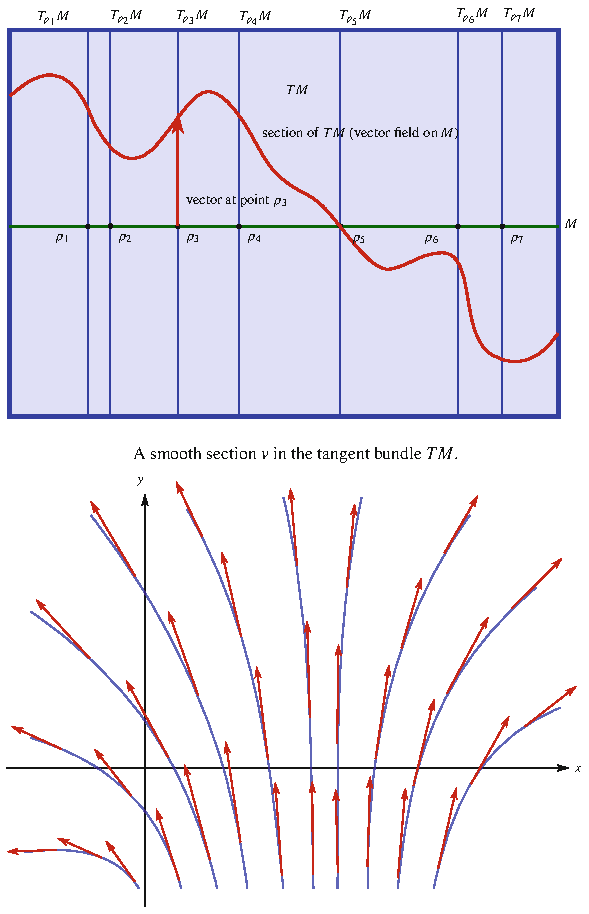
\includegraphics[width=0.757\linewidth]{images/vector/fig-A-1.pdf}
  \caption{切丛 $TM$ 的可积截面 $v$(上图)就是流形 $M$ 上的向量场 $v$, 它在 $M$ 上有积分曲线 $\gamma$(下图)}
  \label{fig:A-1}
\end{figure}

把 $\gamma$ 想成到流形的函数 $\gamma:\mathbb{R}\to M$, 把 $x^i$ 想成流形上的坐标函数 $x^i:M\to\mathbb{R}$, 那么我们也可以把这 $n$ 个微分方程的方程组写成
\[
\frac{d}{dt}x^i\left(\gamma(t)\right)=v^i\left(\gamma(t)\right),
\]
其中 $v^i:M\to\mathbb{R}$ 是向量 $v$ 的实值分量函数. 解这 $n$ 个微分方程的方程组给出组成积分曲线 $\gamma$ 的 $n$ 个积分函数 $\gamma^i$. 见图~\ref{fig:A-2}. 因此, 这种在流形上对向量场积分的思想归结为微分方程.

\begin{figure}[htbp]
  \centering
  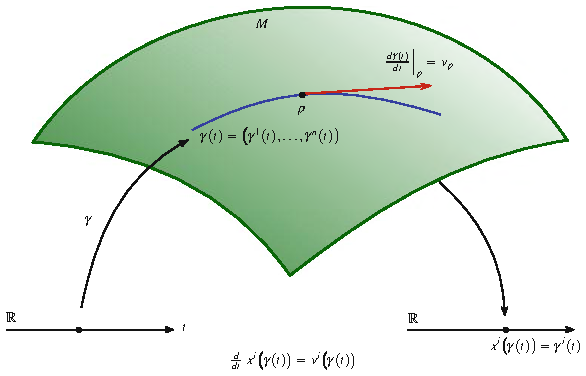
\includegraphics[width=0.764\linewidth]{images/vector/fig-A-2.pdf}
  \caption{流形 $M$ 及其一条积分曲线 $\gamma$, 它通过求解微分方程 $\frac{d}{dt}x^i\left(\gamma(t)\right)=v^i\left(\gamma(t)\right)$ 得到. 本质上, 积分曲线 $\gamma$ 是对向量场 $v$ 积分得到的. 虽然这里只画出一条曲线, 但整个流形 $M$ 都被这些曲线填满}
  \label{fig:A-2}
\end{figure}

积分曲线 $\gamma$ 就是流形 $M$ 上的曲线, 但我们也可以把它们想成从流形 $M$ 到自身、或到 $M$ 的另一个副本的映射族. 我们首先固定某个时间 $t_0$ 作为零时间. 然后对每个时间 $t$ 有一个把 $\gamma(t_0)$ 送到 $\gamma(t_0+t)$ 的映射 $\gamma_t$：
\[
M\overset{\gamma_t}{\longrightarrow}M,\qquad p=\gamma(t_0)\longmapsto\gamma_t(p)=\gamma(t_0+t).
\]
每个不同的时间 $t$ 给出不同的映射 $\gamma_t$, 从而给我们一整族映射, 如图~\ref{fig:A-3} 所示. 一旦我们有了流形之间的映射 $\gamma_t:M\to M$, 就有前推映射
\[
T_p\gamma_t\equiv\gamma_{t*}:T_pM\to T_{\gamma_t(p)}M,
\]
它使我们能够前推向量, 以及拉回映射
\[
T_p^*\gamma_t\equiv\gamma_t^*:T_{\gamma_t(p)}^*M\to T_p^*M,
\]
它使我们能够拉回 1-形式. 我们通常从记号中略去点 $p$, 并从上下文推断. 这样我们就简单地写 $T\gamma_t\equiv\gamma_{t*}$ 与 $T^*\gamma_t\equiv\gamma_t^*$. 见图~\ref{fig:A-4}.

\begin{figure}[htbp]
  \centering
  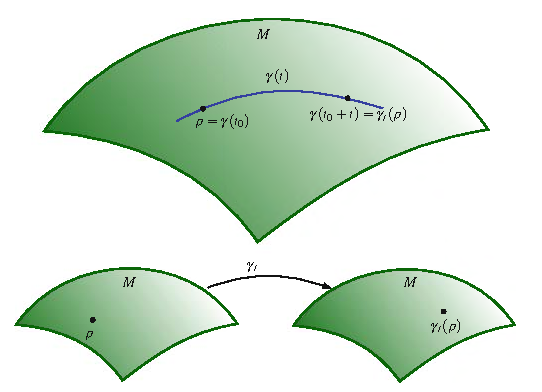
\includegraphics[width=0.694\linewidth]{images/vector/fig-A-3.pdf}
  \caption{对向量场 $v$ 积分得到的积分曲线 $\gamma$ 可用来定义一整族映射 $\gamma_t:M\to M$, 每个 $t$ 值对应一个映射. 映射 $\gamma_t$ 把流形上每个点 $p=\gamma(t_0)$ 送到 $\gamma_t(p)=\gamma(t_0+t)$}
  \label{fig:A-3}
\end{figure}

\begin{figure}[htbp]
  \centering
  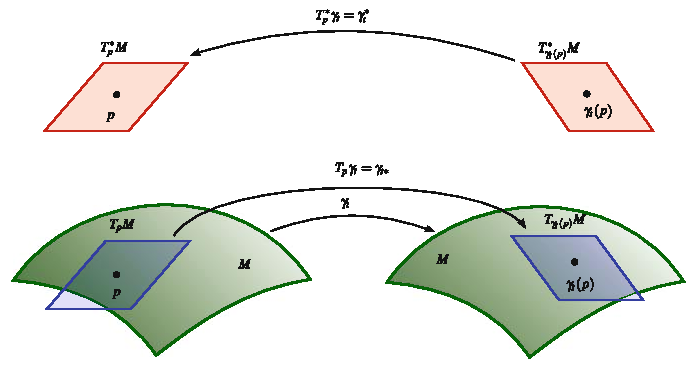
\includegraphics[width=0.960\linewidth]{images/vector/fig-A-4.pdf}
  \caption{映射 $\gamma_t$ 可用来通过 $T_p\gamma_t\equiv\gamma_{t*}$ 前推向量, 并通过 $T_p^*\gamma_t\equiv\gamma_t^*$ 拉回 1-形式}
  \label{fig:A-4}
\end{figure}

当然, 映射 $\gamma_t$ 是可逆的. 假设 $\gamma_t(p)=q$. 那么我们可以定义 $\gamma_t^{-1}(q)=p$. 让我们仔细看看定义：对某个 $t_0$, $p=\gamma(t_0)$ 而 $q=\gamma(t_0+t)$. 我们可以让时间向后跑, 就像向前跑一样容易, 所以如果我们定义 $\tilde{t}_0=t_0+t$, 那么有 $\gamma(\tilde{t}_0)=q$ 与 $\gamma(\tilde{t}_0-t)=p$. 但这正好等同于说 $\gamma_{-t}(q)=p$, 而这正是我们想要 $\gamma_t^{-1}$ 做的. 因此有 $\gamma_t^{-1}=\gamma_{-t}$. 因此我们也可以定义 $\gamma_t^{-1}=\gamma_{-t}$ 的前推与拉回. 我们只需要前推：
\[
T_q\gamma_t^{-1}\equiv T_q\gamma_{-t}\equiv\gamma_{-t*}:T_qM\to T_{\gamma_{-t}(q)}M,
\]
其中当然 $q=\gamma_t(p)$. 从记号中略去点 $q$, 我们写 $T\gamma_t^{-1}\equiv T\gamma_{-t}$, 剩下的基点留给上下文推断.

\subsection{向量场的 Lie 导数}

现在我们可以给出 Lie 导数的定义了. 我们首先给出向量场 $w$ 在 $v$ 方向上的 Lie 导数的定义, 不过也许更准确地说, 它是 $w$ 沿向量场 $v$ 的流的 Lie 导数, 在点 $p$ 处：
\[
\text{向量场的 Lie 导数：}\qquad (L_vw)_p=\lim_{t\to0}\frac{T\gamma_{-t}\cdot w_{\gamma_t(p)}-w_p}{t}.
\]
你当然会遇到向量场的 Lie 导数的相当多种类的记号, 例如
\begin{align*}
(L_vw)_p&=\lim_{t\to0}\frac{\gamma_t^{-1*}w_{\gamma_t(p)}-w_p}{t}\\
&=\lim_{t\to0}\frac{\gamma_{-t*}w_{\gamma_t(p)}-w_p}{t}\\
&=\lim_{t\to0}\frac{\gamma_t^{-1*}w_{\gamma_t(p)}-\gamma_0^{-1*}w_{\gamma_0(p)}}{t}\\
&\equiv\left.\frac{d}{dt}\left(\gamma_t^{-1*}w_{\gamma_t(p)}\right)\right|_{0}\\
&=\left.\frac{d}{dt}\left(\gamma_{-t*}w_{\gamma_t(p)}\right)\right|_{0}.
\end{align*}
（证明这些不同记号表示同一意思参见问题~\ref{q:A-8}.）

这里发生了什么？我们想理解向量场 $w$ 在点 $p$ 处如何变化. 为此我们需要先选择一个方向 $v_p$. 实际上, 我们需要的还多一点点：我们需要定义在点 $p$ 附近的向量场 $v$ 的一小段积分曲线（见图~\ref{fig:A-5}）. 有了它, 我们就能测量向量场 $w$ 沿 $v$ 的积分曲线如何变化. 我们通过 $T\gamma_{-t}$ 把向量 $w_{\gamma_t(p)}$ 拉回到点 $p$ 来做到这一点. 这样 $w_p$ 与 $T\gamma_{-t}\cdot w_{\gamma_t(p)}$ 都是点 $p$ 处的向量, 也就是说, 都是 $T_pM$ 中的向量, 所以我们可以把一个减去另一个, 如图~\ref{fig:A-6} 所示. 这就成为差商的分子, $t$ 是分母. 用数 $t$ 除一个向量, 就是把这个向量的每个分量除以 $t$. 当 $t\to0$ 取极限, 就给出 $w$ 沿 $v$ 在点 $p$ 处的 Lie 导数. 其几何直观如图~\ref{fig:A-5} 所示. 于是我们有：Lie 导数事实上是另一个向量场, 一个我们已经遇到过的向量场. 几页之后会对此多说一些.

\begin{figure}[htbp]
  \centering
  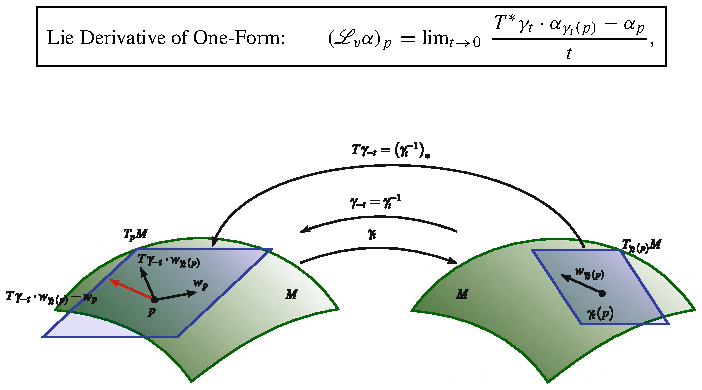
\includegraphics[width=0.832\linewidth]{images/vector/fig-A-5.pdf}
  \caption{为了求向量场 $w$ 在方向 $v$ 上的 Lie 导数，我们首先找到 $v$ 的积分曲线 $\gamma$. 借助 $\gamma$，我们得到一整族映射 $\gamma_t$，它们只需将流形 $M$ 上的点 $p$ 沿流 $\gamma$ 移动时间 $t$，如图~\ref{fig:A-4} 所示. 然后我们可以通过 $T\gamma_{-t}$ 将向量 $w_{\gamma_t(p)}$ 前推到点 $p$，并从中减去 $w_p$. 这构成了 Lie 导数差商的分子.}
  \label{fig:A-5}
\end{figure}

\begin{figure}[htbp]
  \centering
  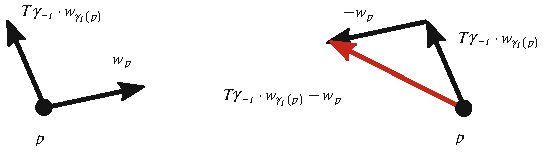
\includegraphics[width=0.838\linewidth]{images/vector/fig-A-6.pdf}
  \caption{这里以几何方式展示如何从向量 $T\gamma_{-t}\cdot w_{\gamma_t(p)}$ 中减去向量 $w_p$，得到向量 $T\gamma_{-t}\cdot w_{\gamma_t(p)}-w_p$.}
  \label{fig:A-6}
\end{figure}

\subsection{1-形式的 Lie 导数}

微分形式 $\alpha$ 在 $v$ 方向上、点 $p$ 处的 Lie 导数以完全相同的方式定义, 只是我们必须用拉回而不是前推：
\[
\text{1-形式的 Lie 导数：}\qquad (L_v\alpha)_p=\lim_{t\to0}\frac{T^*\gamma_t\cdot\alpha_{\gamma_t(p)}-\alpha_p}{t},
\]
它当然也可以写成
\begin{align*}
(L_v\alpha)_p&=\lim_{t\to0}\frac{\gamma_t^*\alpha_{\gamma_t(p)}-\alpha_p}{t}\\
&=\lim_{t\to0}\frac{\gamma_t^*\alpha_{\gamma_t(p)}-\gamma_0^*\alpha_{\gamma_0(p)}}{t}\\
&\equiv\left.\frac{d}{dt}\left(\gamma_t^*\alpha_{\gamma_t(p)}\right)\right|_{0}.
\end{align*}
注意, 1-形式 $\alpha$ 的 Lie 导数与向量场 $w$ 的 Lie 导数完全类似地定义（见图~\ref{fig:A-7}；证明这些记号等价参见问题~\ref{q:A-9}）.

\begin{figure}[htbp]
  \centering
  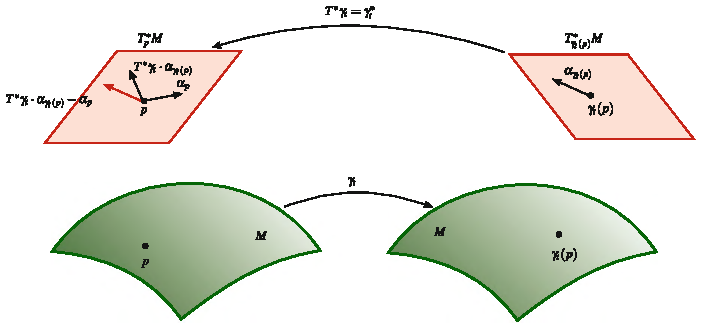
\includegraphics[width=0.960\linewidth]{images/vector/fig-A-7.pdf}
  \caption{为了求 1-形式 $\alpha$ 在方向 $v$ 上的 Lie 导数，我们首先找到 $v$ 的积分曲线 $\gamma$. 借助 $\gamma$，我们得到一整族映射 $\gamma_t$，它们只需将流形 $M$ 上的点 $p$ 沿流 $\gamma$ 移动时间 $t$，如图~\ref{fig:A-4} 所示. 然后我们可以通过 $T^*\gamma_t$ 将 1-形式 $\alpha_{\gamma_t(p)}$ 拉回到点 $p$，并从中减去 $\alpha_p$. 这构成了 Lie 导数差商的分子.}
  \label{fig:A-7}
\end{figure}

\subsection{函数的 Lie 导数}

函数的 Lie 导数会是什么？由于我们之前把函数看成 0-形式, 我们也可以把它们看成零阶协变张量, 并用 1-形式的 Lie 导数公式得到
\[
(L_vf)_p=\lim_{t\to0}\frac{T^*\gamma_t\cdot f_{\gamma_t(p)}-f_p}{t}.
\]
但 $f_{\gamma_t(p)}$ 不过是 $f\left(\gamma_t(p)\right)=f(q)$, 即 $f$ 在 $\gamma_t(p)=q$ 处求值的数值. 一个数被 $\gamma_t^*$ 拉回就是那个数本身, 所以有 $\gamma_t^*f_{\gamma_t(p)}=f\left(\gamma_t(p)\right)=f(q)$. 类似地, $f_p$ 不过是函数 $f$ 在点 $p$ 处求值, 即 $f(p)$. 由于 $p=\gamma(t_0)$, $q=\gamma(t_0+t)$, 把一切合在一起我们可以写
\begin{align*}
(L_vf)_p&=\lim_{t\to0}\frac{f\left(\gamma(t_0+t)\right)-f\left(\gamma(t_0)\right)}{t}\\
&=\left.\frac{\partial f\left(\gamma(t)\right)}{\partial t}\right|_{t_0}\\
&=\left.\frac{\partial f}{\partial\gamma^i}\right|_{\gamma(t_0)}\left.\frac{\partial\gamma^i}{\partial t}\right|_{t_0}.
\end{align*}
最后一个等式不过是链式法则. 积分曲线 $\gamma$ 可以写成 $\gamma(t)=\left(\gamma^1(t),\ldots,\gamma^n(t)\right)$, 但 $\gamma^i$ 是什么？它不过是曲线的 $x^i$ 坐标, 所以我们可以重新标记, 用更标准的记号把曲线写成 $\gamma(t)=\left(x^1(t),\ldots,x^n(t)\right)$. 用更标准的记号重写这条曲线, 只是让我们更容易认出最终结果, 它可以写成
\[
(L_vf)_p=\left.\frac{\partial f}{\partial x^i}\right|_{\gamma(t_0)}\left.\frac{\partial x^i}{\partial t}\right|_{t_0}.
\]
接下来回忆我们当初是如何得到 $x^i$ 坐标 $\gamma^i$ 的：我们通过解微分方程组
\[
\frac{d}{dt}\gamma^i=v^i
\]
从向量 $v$ 得到它, 从而给出
\begin{align*}
(L_vf)_p&=\frac{\partial f}{\partial x^i}v^i\\
&=v^i\frac{\partial f}{\partial x^i}\\
&=v^i\frac{\partial}{\partial x^i}f\\
&=v_p[f],
\end{align*}
这不过是 $f$ 在 $v$ 方向上的方向导数. 所以对函数而言, Lie 导数与我们熟悉的方向导数没有区别. 于是我们得到
\[
\text{函数的 Lie 导数：}\qquad (L_vf)_p=v_p[f].
\]

\subsection{$(r,s)$-型张量的 Lie 导数}

现在我们转向 $(r,s)$-型张量 $T$ 的 Lie 导数. 我们用下式定义张量 $T$ 被 $\gamma_t$ 的拉回：
\[
\left(\gamma_t^*T\right)_p\left(\alpha_1,\ldots,\alpha_r,v_1,\ldots,v_s\right)
=T_{\gamma_t(p)}\left(\gamma_{-t}^*\alpha_1,\ldots,\gamma_{-t}^*\alpha_r,\gamma_{t*}v_1,\ldots,\gamma_{t*}v_s\right).
\]
把它与我们对 1-形式的拉回的原始定义比较. 这样定义张量的拉回, 我们用与定义 1-形式的 Lie 导数相同的公式定义张量 $T$ 的 Lie 导数：
\[
\text{张量的 Lie 导数：}\qquad (L_vT)_p=\lim_{t\to0}\frac{\gamma_t^*T_{\gamma_t(p)}-T_p}{t}.
\]
当然我们也可以把一般张量场的 Lie 导数写成
\begin{align*}
(L_vT)_p&=\lim_{t\to0}\frac{\gamma_t^*T_{\gamma_t(p)}-\gamma_0^*T_{\gamma_0(p)}}{t}\\
&=\left.\frac{d}{dt}\left(\gamma_t^*T_{\gamma_t(p)}\right)\right|_{0}.
\end{align*}

\subsection{若干 Lie 导数恒等式}

现在我们转向证明若干涉及 Lie 导数的重要恒等式. 我们相当快速地过一遍这些恒等式, 把一些留作练习. 第一个恒等式是：无论张量 $S$ 和 $T$ 属于哪种类型, Lie 导数都是线性的. 也就是说, 对 $a,b\in\mathbb{R}$, 有
\[
L_v\left(aS+bT\right)=aL_vS+bL_vT.
\]
转向两个张量的张量积的 Lie 导数, 并从记号中略去基点、依赖恒等式 $\varphi^*\left(T\otimes S\right)=\varphi^*T\otimes\varphi^*S$, 我们发现
\begin{align*}
L_v(S\otimes T)&=\lim_{t\to0}\frac{\gamma_t^*(S\otimes T)-S\otimes T}{t}\\
&=\lim_{t\to0}\frac{\gamma_t^*S\otimes\gamma_t^*T-S\otimes T}{t}\\
&=\lim_{t\to0}\frac{\left(S+(\gamma_t^*S-S)\right)\otimes\left(T+(\gamma_t^*T-T)\right)-S\otimes T}{t}\\
&=\lim_{t\to0}\frac{(\gamma_t^*S-S)\otimes T+S\otimes(\gamma_t^*T-T)+(\gamma_t^*S-S)\otimes(\gamma_t^*T-T)}{t}\\
&=\lim_{t\to0}\frac{\gamma_t^*S-S}{t}\otimes T+\lim_{t\to0}S\otimes\frac{\gamma_t^*T-T}{t}+\lim_{t\to0}\frac{\gamma_t^*S-S}{t}\otimes(\gamma_t^*T-T)\\
&=L_vS\otimes T+S\otimes L_vT+L_vS\otimes0\\
&=L_vS\otimes T+S\otimes L_vT.
\end{align*}
显然, 在倒数第二行中, 当 $t\to0$ 时, 有 $(\gamma_t^*T-T)\to(T-T)=0$. 其中一步极限交换的合理性留作问题~\ref{q:A-12}.

把一切合在一起, 我们证明了恒等式
\[
L_v(S\otimes T)=L_vS\otimes T+S\otimes L_vT.
\]
类似地, 依赖第 6.7 节的恒等式 $\varphi^*(\alpha\wedge\beta)=\varphi^*\alpha\wedge\varphi^*\beta$, 我们有
\begin{align*}
L_v(\alpha\wedge\beta)&=\lim_{t\to0}\frac{\gamma_t^*(\alpha\wedge\beta)-\alpha\wedge\beta}{t}\\
&=\lim_{t\to0}\frac{\gamma_t^*\alpha\wedge\gamma_t^*\beta-\alpha\wedge\beta}{t}\\
&=\lim_{t\to0}\frac{\left(\alpha+(\gamma_t^*\alpha-\alpha)\right)\wedge\left(\beta+(\gamma_t^*\beta-\beta)\right)-\alpha\wedge\beta}{t}\\
&=\lim_{t\to0}\frac{(\gamma_t^*\alpha-\alpha)\wedge\beta+\alpha\wedge(\gamma_t^*\beta-\beta)+(\gamma_t^*\alpha-\alpha)\wedge(\gamma_t^*\beta-\beta)}{t}\\
&=\lim_{t\to0}\frac{\gamma_t^*\alpha-\alpha}{t}\wedge\beta+\lim_{t\to0}\alpha\wedge\frac{\gamma_t^*\beta-\beta}{t}+\lim_{t\to0}\frac{\gamma_t^*\alpha-\alpha}{t}\wedge(\gamma_t^*\beta-\beta)\\
&=L_v\alpha\wedge\beta+\alpha\wedge L_v\beta+L_v\alpha\wedge0\\
&=L_v\alpha\wedge\beta+\alpha\wedge L_v\beta.
\end{align*}
同样, 显然在倒数第二行中, 当 $t\to0$ 时, 有 $(\gamma_t^*\beta-\beta)\to(\beta-\beta)=0$. 其中一步极限交换的合理性留作问题~\ref{q:A-13}.

把一切合在一起, 我们证明了恒等式
\[
L_v(\alpha\wedge\beta)=L_v\alpha\wedge\beta+\alpha\wedge L_v\beta.
\]
下一个恒等式涉及函数 $f$ 与向量场 $v$ 和 $w$. 它是
\[
L_v(fw)=fL_vw+v[f]w.
\]
另一个重要的恒等式是
\[
d\left(L_v\alpha\right)=L_v\left(d\alpha\right).
\]
这来自拉回与外微分的可交换性 $\varphi^*d=d\varphi^*$(见问题~\ref{q:A-15}).

\subsection{Cartan 同伦公式}

我们现在证明一个非常重要的恒等式, 称为 Cartan 同伦公式, 有时也叫 Cartan 魔术公式. 给定 $k$-形式 $\alpha$ 与向量场 $v$, 并回忆第 3.4 节内积 $\iota$ 的定义, Cartan 魔术公式是
\[
L_v\alpha=\iota_v(d\alpha)+d(\iota_v\alpha).
\]
虽然有好几种方式证明这个恒等式, 我们将使用归纳法. 首先考虑零形式 $\alpha=f$ 的基础情形. 内积 $\iota_vf$ 对零形式没有定义, 所以恒等式简化为
\[
L_vf=\iota_v(df).
\]
但这显然是真的, 只要你记得所有写同一件事的不同方式. 回忆我们求得函数的 Lie 导数就是函数的方向导数, 即 $L_vf=v[f]$. 还回忆本书早些时候 $v[f]\equiv df(v)$, 当然按内积的定义 $df(v)=\iota_vdf$. 于是我们得到下面这串等式, 它们不过是用不同的方式写同一件事：
\[
L_vf=v[f]=df(v)=\iota_vdf.
\]
这个"通过记号证明"的经典例子确立了我们的基础情形. 还请注意, 如果函数 $f$ 是坐标函数 $x^i$, 那么有 $L_vx^i=\iota_vdx^i$. 一会儿我们将需要这个事实.

现在假设恒等式 $L_v\alpha=\iota_v(d\alpha)+d(\iota_v\alpha)$ 对所有 $(k-1)$-形式 $\alpha$ 成立. 假设我们有 $k$-形式 $\omega=fdx^1\wedge\cdots\wedge dx^k$, 它显然是 $k$-形式的一般基底项. 我们可以把 $\omega$ 写成 $\omega=dx^1\wedge\alpha$, 其中 $\alpha=fdx^2\wedge\cdots\wedge dx^k$ 是 $(k-1)$-形式. 回忆我们刚证明的恒等式之一, Cartan 魔术公式的左边变成
\[
L_v\omega=L_v(dx^1\wedge\alpha)=L_vdx^1\wedge\alpha+dx^1\wedge L_v\alpha.
\]
在转向 Cartan 魔术公式的右边之前, 我们回忆几个将需要的恒等式. 第一个是第 3.4 节证明的内积恒等式. 如果 $\alpha$ 是 $k$-形式而 $\beta$ 是另一个微分形式, 那么
\[
\iota_v(\alpha\wedge\beta)=(\iota_v\alpha)\wedge\beta+(-1)^k\alpha\wedge(\iota_v\beta)
=\iota_v\alpha\wedge\beta+(-1)^k\alpha\wedge\iota_v\beta.
\]
第二个是外导数的恒等式. 这个恒等式要么作为我们定义外导数方式的推论被导出, 如第 4.2 节；要么被视为允许我们找出外导数公式的外微分公理, 如第 4.3 节. 如果 $\alpha$ 是 $k$-形式而 $\beta$ 是另一个微分形式, 那么
\[
d(\alpha\wedge\beta)=(d\alpha)\wedge\beta+(-1)^k\alpha\wedge(d\beta)
=d\alpha\wedge\beta+(-1)^k\alpha\wedge d\beta.
\]
现在我们考虑 Cartan 魔术公式的右边：
\begin{align*}
\iota_v(d\omega)+d(\iota_v\omega)&=\iota_v\left(d(dx^1\wedge\alpha)\right)+d\left(\iota_v(dx^1\wedge\alpha)\right)\\
&=\iota_v\left(\underbrace{ddx^1}_{=0}\wedge\alpha+(-1)^1dx^1\wedge d\alpha\right)+d\left(\iota_vdx^1\wedge\alpha+(-1)^1dx^1\wedge\iota_v\alpha\right)\\
&=-\iota_vdx^1\wedge d\alpha+d\left(\iota_vdx^1\wedge\alpha\right)-d\left(dx^1\wedge\iota_v\alpha\right)\\
&=-\iota_vdx^1\wedge d\alpha+dx^1\wedge\iota_vd\alpha+d\left(\iota_vdx^1\right)\wedge\alpha+(-1)^0\iota_vdx^1\wedge d\alpha\\
&\quad-\underbrace{d(dx^1)}_{=0}\wedge\iota_v\alpha-(-1)^1dx^1\wedge d(\iota_v\alpha)\\
&=d\left(L_vx^1\right)\wedge\alpha+dx^1\wedge\iota_vd\alpha+dx^1\wedge d(\iota_v\alpha)\\
&=L_vdx^1\wedge\alpha+dx^1\wedge\left(\iota_vd\alpha+d\iota_v\alpha\right)\\
&=L_vdx^1\wedge\alpha+dx^1\wedge L_v\alpha.
\end{align*}
其中倒数第二步用到了恒等式 $d(L_vx^1)=L_v(dx^1)$(问题~\ref{q:A-15}), 最后一步用到了对 $(k-1)$-形式 $\alpha$ 的归纳假设. 所以对于 $\omega=dx^1\wedge\alpha$, Cartan 魔术公式的左边和右边都等于同一个东西, 即 $L_vdx^1\wedge\alpha+dx^1\wedge L_v\alpha$, 因而彼此相等.

利用外微分、Lie 导数与内积的线性性, 可以把这一证明推广到一切形如 $\omega=\sum f_{i_1\cdots i_k}dx^{i_1}\wedge\cdots\wedge dx^{i_k}$ 的微分形式(见问题~\ref{q:A-16}). 于是我们已对任意微分形式 $\alpha$ 证明了
\[
\text{Cartan 同伦公式：}\qquad L_v\alpha=\iota_v(d\alpha)+d(\iota_v\alpha).
\]
这个恒等式常常就简单地写为 $L_v=\iota_vd+d\iota_v$.

\subsection{Lie 导数等于交换子}

现在我们注意转向证明：向量场 $w$ 在 $v$ 方向上的 Lie 导数等于 $v$ 与 $w$ 的交换子. 换言之, 我们将证明恒等式
\[
L_vw=[v,w]=vw-wv.
\]
我们第一次遇到 $v$ 与 $w$ 的交换子(也称为 $v$ 与 $w$ 的 Lie 括号)是在第 4.4.2 小节, 当时我们试图从某种几何的角度解释 $[v,w]$ 是什么. 这个恒等式的证明几乎过于流畅, 不过是用定义与记号进行一些巧妙操作.

首先考虑这样的情形：有映射 $\varphi:M\to N$、$M$ 上的向量 $w_p$ 以及实值函数 $f:N\to\mathbb{R}$. 我们可以用 $\varphi$ 把 $M$ 上的向量 $w_p$ 前推到 $N$ 上的向量 $T_p\varphi\cdot w_p$. 然后可以求 $f$ 在点 $\varphi(p)$ 处沿方向 $T_p\varphi\cdot w_p$ 的方向导数. 这是一个数值. 按定义, 向量被映射 $\varphi$ 的前推作用于函数 $f$, 给出与向量在点 $p$ 处作用于 $f\circ\varphi$ 相同的数值, 即
\[
w_p\left[f\circ\varphi\right]=\left(T_p\varphi\cdot w_p\right)_{\varphi(p)}[f].
\]
我们重申, 作为数值它们是相等的. 但如我们所知, 函数的导数是另一个函数, 只有当我们把这个函数在某点求值时才能得到数值. 如果 $w$ 实际上是 $M$ 上的向量场, 那么 $w[f\circ\varphi]$ 是 $M$ 上的函数. 类似地, $\left(T\varphi\cdot w\right)[f]$ 是 $N$ 上的函数. 但显然, 由于这两个函数甚至不在同一个流形上, 
\[
w[f\circ\varphi]\neq\left(T\varphi\cdot w\right)[f].
\]
我们如何修复？由于 $\left(T\varphi\cdot w\right)[f]$ 是 $N$ 上的函数, 它不过是一个零形式, 我们可以把它拉回到 $M$. 回忆零形式的拉回是如何定义的, 有
\[
T^*\varphi\cdot\left(\left(T\varphi\cdot w\right)[f]\right)=\left(T\varphi\cdot w\right)[f]\circ\varphi,
\]
它现在是 $M$ 上的函数, 给出与 $w[f\circ\varphi]$ 相同的数值, 我们也可以把它改写为 $w\left[T^*\varphi\cdot f\right]$（见图~\ref{fig:A-8}）. 于是我们最终得到 $M$ 上函数的相当漂亮的等式
\[
w\left[T^*\varphi\cdot f\right]=T^*\varphi\cdot\left(\left(T\varphi\cdot w\right)[f]\right).
\]
这个过程说明了我们需要使用的一般思想.

\begin{figure}[htbp]
  \centering
  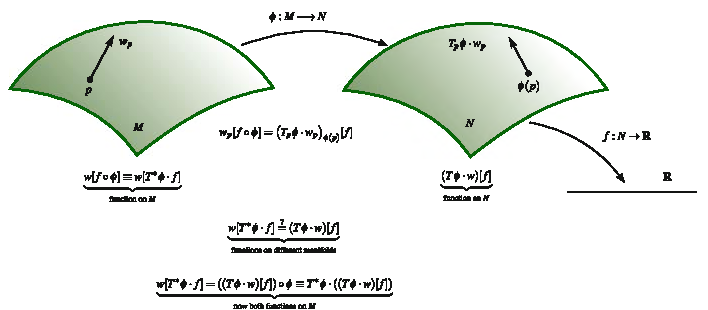
\includegraphics[width=0.960\linewidth]{images/vector/fig-A-8.pdf}
  \caption{由第 10.3 节的一个问题可知 $w_p[f\circ\varphi]=(T_p\varphi\cdot w_p)_{\varphi(p)}[f]$. 但这是数值的等式. 去掉基点后右边变成 $w[f\circ\varphi]$，即 $f\circ\varphi$ 在 $w$ 方向上的方向导数，它本身是 $M$ 上的函数. 类似地，左边变成 $(T\varphi\cdot w)[f]$，即 $f$ 在 $T\varphi\cdot w$ 方向上的方向导数，它本身是 $N$ 上的函数. 从而 $w[f\circ\varphi]$ 与 $(T\varphi\cdot w)[f]$ 作为函数不能相等. 但这可以通过用 $T^*\varphi$ 拉回零形式（函数）$(T\varphi\cdot w)[f]$ 来解决. 零形式的拉回也定义在第 10.3 节.}
  \label{fig:A-8}
\end{figure}

现在我们考虑与我们有关的特定情形. 假设 $M$ 上有可积向量场 $v$, 其积分曲线 $\gamma$ 以时间 $t$ 为参数. 那么对每个时间 $t$ 我们得到一个映射 $\gamma(t):M\to\widetilde{M}$, 其中我们简单地让值域流形 $\widetilde{M}=M$. 我们可以让时间倒流得到逆映射 $(\gamma_t)^{-1}=\gamma_{-t}:\widetilde{M}\to M$. 现在假设 $M=\widetilde{M}$ 上有向量场 $w$, 并有实值映射 $f:M\to\mathbb{R}$, 见图~\ref{fig:A-9}. 我们有以下数值相等：
\[
\left(T_{\gamma_t(p)}\gamma_{-t}\cdot w_{\gamma_t(p)}\right)_p[f]=w_{\gamma_t(p)}\left[f\circ\gamma_{-t}\right].
\]
但如果去掉基点, 等式两边就不再是数值而是函数：左边 $\left(T\gamma_{-t}\cdot w\right)[f]$ 是 $\widetilde{M}$ 上的函数, 右边 $w[f\circ\gamma_{-t}]$ 是 $M$ 上的函数. 为了得到函数之间的等式, 我们可以在 $M$ 上拉回右边, 得到 $M$ 上函数的等式
\[
\left(T\gamma_{-t}\cdot w\right)[f]=\left(w\left[f\circ\gamma_{-t}\right]\right)\circ\gamma_t,
\]
它也可以改写为
\[
\left(T\gamma_{-t}\cdot w\right)[f]=T^*\gamma_t\cdot\left(w\left[T^*\gamma_{-t}\cdot f\right]\right).
\]
这正是我们需要的恒等式.

\begin{figure}[htbp]
  \centering
  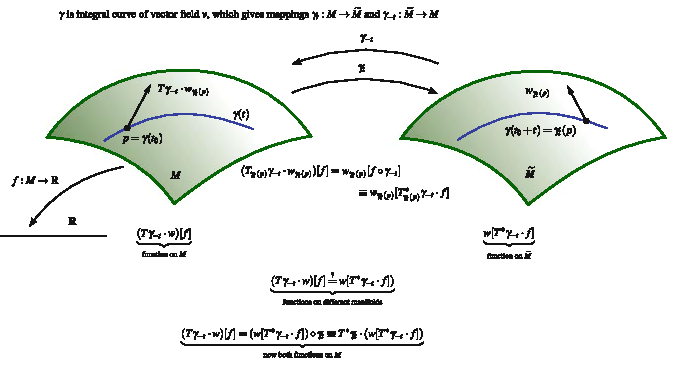
\includegraphics[width=0.940\linewidth]{images/vector/fig-A-9.pdf}
  \caption{这里类似于图~\ref{fig:A-8} 的过程使我们能够使 $M$ 上的两个函数相等，从而得到 $(T\gamma_{-t}\cdot w)[f]=T^*\gamma_t\cdot(w[T^*\gamma_{-t}\cdot f])$. 这正是我们在证明 $L_vw=[v,w]$ 时需要的特定情形.}
  \label{fig:A-9}
\end{figure}

现在我们终于准备好证明 $L_vw=[v,w]=vw-wv$. 我们首先写出向量场 $w$ 在 $v$ 方向上的 Lie 导数的定义：
\[
(L_vw)_p=\lim_{t\to0}\frac{T\gamma_{-t}\cdot w_{\gamma_t(p)}-w_p}{t}.
\]
由于我们感兴趣的是独立于基点 $p$ 的一般公式, 我们将使用不带基点的这个定义. 如果你想放回基点, 就需要仔细考虑向量 $w$ 位于何处. 此外, 由于 $L_vw$ 本身是向量场, 我们可以用它来求函数 $f$ 的方向导数, 所以有
\begin{align*}
\left(L_vw\right)[f]&=\lim_{t\to0}\frac{T\gamma_{-t}\cdot w-w}{t}[f]\\
&=\lim_{t\to0}\frac{\left(T\gamma_{-t}\cdot w\right)[f]-w[f]}{t}\\
&=\lim_{t\to0}\frac{T^*\gamma_t\cdot\left(w\left[T^*\gamma_{-t}\cdot f\right]\right)-w[f]}{t}\\
&=\lim_{t\to0}\frac{T^*\gamma_t\cdot\left(w\left[T^*\gamma_{-t}\cdot f\right]\right)-T^*\gamma_t\cdot w[f]+T^*\gamma_t\cdot w[f]-w[f]}{t}\\
&=\lim_{t\to0}\frac{T^*\gamma_t\cdot\left(w\left[T^*\gamma_{-t}\cdot f\right]\right)-T^*\gamma_t\cdot w[f]}{t}+\lim_{t\to0}\frac{T^*\gamma_t\cdot w[f]-w[f]}{t}\\
&=\lim_{t\to0}T^*\gamma_t\cdot w\left(\frac{T^*\gamma_{-t}\cdot f-f}{t}\right)+\lim_{t\to0}\frac{T^*\gamma_t\cdot w[f]-w[f]}{t}\\
&=\lim_{t\to0}T^*\gamma_t\cdot w\left(\frac{f\circ\gamma_{-t}-f}{t}\right)+\lim_{t\to0}\frac{w[f]\circ\gamma_t-w[f]}{t}\\
&=T^*\gamma_0\cdot\left(w\left[-v[f]\right]\right)+v\left[w[f]\right]\\
&=-w\left[v[f]\right]+v\left[w[f]\right]\\
&=[v,w]f.
\end{align*}
其中第三步用了恒等式 $\left(T\gamma_{-t}\cdot w\right)[f]=T^*\gamma_t\cdot\left(w\left[T^*\gamma_{-t}\cdot f\right]\right)$(问题~\ref{q:A-17}), 倒数第二步用了问题~\ref{q:A-18} 与问题~\ref{q:A-19} 的结果. 去掉函数 $f$ 就给出 $L_vw=[v,w]=vw-wv$.

这里我们花点时间写下交换子的一个公式. 假设 $v=\sum v^i\frac{\partial}{\partial x^i}=v^i\frac{\partial}{\partial x^i}$, $w=\sum w^j\frac{\partial}{\partial x^j}=w^j\frac{\partial}{\partial x^j}$. Lie 导数 $L_vw$ 本身是向量场, 因此它可以作用于函数 $f$；也就是说, 我们可以求 $L_vw[f]$, 即 $f$ 在方向 $L_vw$ 上的方向导数. 这个恒等式的意思是
\begin{align*}
L_vw[f]&=v\left[w[f]\right]-w\left[v[f]\right]\\
&=v\left(w^j\frac{\partial}{\partial x^j}[f]\right)-w\left(v^i\frac{\partial}{\partial x^i}[f]\right)\\
&=v\left(w^j\frac{\partial f}{\partial x^j}\right)-w\left(v^i\frac{\partial f}{\partial x^i}\right)\\
&=v^i\frac{\partial}{\partial x^i}\left(w^j\frac{\partial f}{\partial x^j}\right)-w^j\frac{\partial}{\partial x^j}\left(v^i\frac{\partial f}{\partial x^i}\right)\\
&=v^i\frac{\partial w^j}{\partial x^i}\frac{\partial f}{\partial x^j}+v^iw^j\frac{\partial^2f}{\partial x^i\partial x^j}-w^j\frac{\partial v^i}{\partial x^j}\frac{\partial f}{\partial x^i}-w^jv^i\frac{\partial^2f}{\partial x^j\partial x^i}\\
&=v^i\frac{\partial w^j}{\partial x^i}\frac{\partial f}{\partial x^j}-w^j\frac{\partial v^i}{\partial x^j}\frac{\partial f}{\partial x^i}\\
&=\left(v^i\frac{\partial w^j}{\partial x^i}\frac{\partial}{\partial x^j}-w^j\frac{\partial v^i}{\partial x^j}\frac{\partial}{\partial x^i}\right)f.
\end{align*}
因此我们也可以写
\[
L_vw=v^i\frac{\partial w^j}{\partial x^i}\frac{\partial}{\partial x^j}-w^j\frac{\partial v^i}{\partial x^j}\frac{\partial}{\partial x^i}.
\]

\subsection{微分形式 Lie 导数的整体公式}

现在我们转向微分形式的 Lie 导数的整体公式. 这个公式将用于外微分整体公式的证明. 微分形式的 Lie 导数的整体公式由下式给出：
\[
\left(L_v\alpha\right)(w_1,\ldots,w_k)=v\left[\alpha(w_1,\ldots,w_k)\right]-\sum_{i=1}^{k}\alpha\left(w_1,\ldots,[v,w_i],\ldots,w_k\right).
\]
我们将实际执行 2-形式情形的证明, 把一般情形留作练习. 除记号上更复杂外, 一般情形与 2-形式情形类似. 设 $\gamma$ 是 $v$ 的积分曲线, $\alpha$ 是 2-形式, $w_1,w_2$ 是向量场, 我们注意到 $\alpha(w_1,w_2)$ 是函数. 于是有
\begin{align*}
\left(L_v\alpha(w_1,w_2)\right)_p&=\lim_{t\to0}\frac{T^*\gamma_t\left(\alpha(w_1,w_2)\right)_{\gamma_t(p)}-\left(\alpha(w_1,w_2)\right)_p}{t}\\
&=\lim_{t\to0}\frac{\alpha_{\gamma_t(p)}\left(w_{1\gamma_t(p)},w_{2\gamma_t(p)}\right)-\alpha_p\left(w_{1p},w_{2p}\right)}{t}\\
&=\lim_{t\to0}\frac{\alpha_{\gamma_t(p)}\left(w_{1\gamma_t(p)},w_{2\gamma_t(p)}\right)-\alpha_p\left(T\gamma_{-t}\cdot w_{1\gamma_t(p)},T\gamma_{-t}\cdot w_{2\gamma_t(p)}\right)}{t}\\
&\quad+\lim_{t\to0}\frac{\alpha_p\left(T\gamma_{-t}\cdot w_{1\gamma_t(p)},T\gamma_{-t}\cdot w_{2\gamma_t(p)}\right)-\alpha_p\left(w_{1p},T\gamma_{-t}\cdot w_{2\gamma_t(p)}\right)}{t}\\
&\quad+\lim_{t\to0}\frac{\alpha_p\left(w_{1p},T\gamma_{-t}\cdot w_{2\gamma_t(p)}\right)-\alpha_p\left(w_{1p},w_{2p}\right)}{t}.
\end{align*}
最后一个等式后的第一项给出
\begin{align*}
&\lim_{t\to0}\frac{\alpha_{\gamma_t(p)}\left(w_{1\gamma_t(p)},w_{2\gamma_t(p)}\right)-\alpha_p\left(T\gamma_{-t}\cdot w_{1\gamma_t(p)},T\gamma_{-t}\cdot w_{2\gamma_t(p)}\right)}{t}\\
&\qquad=\lim_{t\to0}\frac{T^*\gamma_t\cdot\alpha_{\gamma_t(p)}\left(T\gamma_{-t}\cdot w_{1\gamma_t(p)},T\gamma_{-t}\cdot w_{2\gamma_t(p)}\right)-\alpha_p\left(T\gamma_{-t}\cdot w_{1\gamma_t(p)},T\gamma_{-t}\cdot w_{2\gamma_t(p)}\right)}{t}\\
&\qquad=\lim_{t\to0}\frac{T^*\gamma_t\cdot\alpha_{\gamma_t(p)}-\alpha_p}{t}\left(T\gamma_{-t}\cdot w_{1\gamma_t(p)},T\gamma_{-t}\cdot w_{2\gamma_t(p)}\right)\\
&\qquad=\left(L_v\alpha\right)_p\left(w_{1p},w_{2p}\right).
\end{align*}
最后一个等式后的第二项给出
\begin{align*}
&\lim_{t\to0}\frac{\alpha_p\left(T\gamma_{-t}\cdot w_{1\gamma_t(p)},T\gamma_{-t}\cdot w_{2\gamma_t(p)}\right)-\alpha_p\left(w_{1p},T\gamma_{-t}\cdot w_{2\gamma_t(p)}\right)}{t}\\
&\qquad=\lim_{t\to0}\alpha_p\left(\frac{T\gamma_{-t}\cdot w_{1\gamma_t(p)}-w_{1p}}{t},T\gamma_{-t}\cdot w_{2\gamma_t(p)}\right)\\
&\qquad=\alpha_p\left(\left(L_vw_1\right)_p,w_{2p}\right).
\end{align*}
最后一个等式后的第三项非常类似, 给出
\begin{align*}
&\lim_{t\to0}\frac{\alpha_p\left(w_{1p},T\gamma_{-t}\cdot w_{2\gamma_t(p)}\right)-\alpha_p\left(w_{1p},w_{2p}\right)}{t}\\
&\qquad=\lim_{t\to0}\alpha_p\left(w_{1p},\frac{T\gamma_{-t}\cdot w_{2\gamma_t(p)}-w_{2p}}{t}\right)\\
&\qquad=\alpha_p\left(w_{1p},\left(L_vw_2\right)_p\right).
\end{align*}
于是, 略去基点, 我们有
\[
L_v\alpha(w_1,w_2)=\left(L_v\alpha\right)(w_1,w_2)+\alpha(L_vw_1,w_2)+\alpha(w_1,L_vw_2).
\]
这可以改写为
\[
\left(L_v\alpha\right)(w_1,w_2)=L_v\underbrace{\alpha(w_1,w_2)}_{\text{一个函数}}-\alpha(L_vw_1,w_2)-\alpha(w_1,L_vw_2).
\]
回忆函数的 Lie 导数的定义与 Lie 导数交换子恒等式, 这又可以改写为
\[
\left(L_v\alpha\right)(w_1,w_2)=v\left[\alpha(w_1,w_2)\right]-\alpha([v,w_1],w_2)-\alpha(w_1,[v,w_2]).
\]
这就是 2-形式的 Lie 导数的整体公式.

\begin{center}
\fbox{\parbox{0.86\textwidth}{\centering
微分形式的整体 Lie 导数公式：
\[
\left(L_v\alpha\right)(w_1,\ldots,w_k)=v\left[\alpha(w_1,\ldots,w_k)\right]-\sum_{i=1}^{k}\alpha\left(w_1,\ldots,[v,w_i],\ldots,w_k\right)
\]
}}
\end{center}

一般的 $(r,s)$-型张量 $T$ 的整体 Lie 导数公式由下式给出：
\begin{center}
\fbox{\parbox{0.86\textwidth}{\centering
$(r,s)$-型张量的整体 Lie 导数公式：
\begin{align*}
\left(L_vT\right)(\alpha_1,\ldots,\alpha_r,w_1,\ldots,w_s)
&=v\left[T(\alpha_1,\ldots,\alpha_r,w_1,\ldots,w_s)\right]\\
&\quad-\sum_{i=1}^{r}T\left(\alpha_1,\ldots,L_v\alpha_i,\ldots,\alpha_r,w_1,\ldots,w_s\right)\\
&\quad-\sum_{i=1}^{s}T\left(\alpha_1,\ldots,\alpha_r,w_1,\ldots,L_vw_i,\ldots,w_s\right)
\end{align*}
}}
\end{center}

\subsection{外微分的整体公式}

实际上还有相当多的涉及 Lie 导数的其他重要恒等式与公式, 如果这是微分几何的完整课程, 它们都需要被给出并证明. 然而, 我们将略过它们. 我们现在已经足够详细地覆盖了 Lie 导数, 使你对它们是什么有了基本的理解. 我们现在将以探索 Lie 导数与外微分之间的关系来结束本附录. 由于外微分只适用于微分形式, 即反对称协变张量, 那么显然, 在某种意义上 Lie 导数比外微分更一般, 因为你可以取任何种类的张量的 Lie 导数.

让我们再看一眼 Cartan 魔术公式：
\[
L_v\alpha=\iota_v(d\alpha)+d(\iota_v\alpha).
\]
$k$-形式 $\alpha$ 沿 $v$ 的流的 Lie 导数, 等于 $\alpha$ 的外微分与 $v$ 的内积, 加上 $\alpha$ 与 $v$ 的内积的外微分. 换言之, Cartan 魔术公式使我们能用 $\alpha$ 的外导数写出 $\alpha$ 的 Lie 导数. 于是我们开始看到这两种导数之间确实有关系.

问题是, 我们能反过来, 用 Lie 导数写出外导数吗？答案当然是可以, 但要用向量场的 Lie 导数, 而不是 $k$-形式的. 事实上, 这个公式也称为外微分的整体公式, 在第 4.4.2 小节给出过. 一般 $k$-形式的外微分整体公式的证明需要归纳法. 我们首先证明 1-形式 $\alpha$ 的公式：
\[
d\alpha(v,w)=v[\alpha(w)]-w[\alpha(v)]-\alpha\left([v,w]\right)
=v\alpha(w)-w\alpha(v)-\alpha\left([v,w]\right).
\]
只需假设我们在单个坐标片中, 所以一般 1-形式写成 $\alpha=\sum f_idx^i$. 由于上述方程的两边都是线性的, 我们只需对单项 $f_idx^i$ 证明方程(线性性见问题~\ref{q:A-22}). 但记住 $x^i$ 不过是坐标函数. 为简单起见, 我们将证明 1-形式 $\alpha=fdg$ 的方程, 其中 $f$ 与 $g$ 都是流形上的函数. 于是有
\begin{align*}
d\alpha(v,w)&=d(fdg)(v,w)\\
&=\left(df\wedge dg\right)(v,w)\\
&=df(v)dg(w)-df(w)dg(v)\\
&=v[f]\cdot w[g]-w[f]\cdot v[g]\\
&=(vf)(wg)-(wf)(vg).
\end{align*}
接下来我们看项 $v\alpha(w)$：
\begin{align*}
v\alpha(w)&=v\left(fdg\right)(w)\\
&=v\left(fdg(w)\right)\\
&=v\left(f\cdot w[g]\right)\\
&=v[f]\cdot w[g]+f\cdot v\left[w[g]\right]\qquad\text{乘积法则}\\
&=(vf)(wg)+f\cdot vwg.
\end{align*}
类似地有 $w\alpha(v)=(wf)(vg)+f\cdot wvg$. 由于 $[v,w]=vw-wv$, 我们还有
\begin{align*}
\alpha\left([v,w]\right)&=(fdg)\left([v,w]\right)\\
&=f\cdot[v,w][g]\\
&=f\cdot(vw-wv)[g]\\
&=f\cdot vw[g]-f\cdot wv[g]\\
&=f\cdot vwg-f\cdot wvg.
\end{align*}
把一切合在一起, 有
\begin{align*}
v\alpha(w)-w\alpha(v)-\alpha\left([v,w]\right)
&=(vf)(wg)+f\cdot vwg\\
&\quad-(wf)(vg)-f\cdot wvg\\
&\quad-f\cdot vwg+f\cdot wvg\\
&=(vf)(wg)-(wf)(vg)\\
&=d\alpha(v,w),
\end{align*}
这正是我们想证明的恒等式. 这个恒等式是外导数整体公式的基础情形. 注意我们当然也可以用 Lie 导数写它：
\[
d\alpha(v,w)=v\alpha(w)-w\alpha(v)-\alpha\left(L_vw\right).
\]
当然, 如果我们令 $g=x^i$(坐标函数), 然后使用你在上一个问题中证明的线性性, 就可以看到这个公式适用于所有 1-形式 $\alpha=\sum f_idx^i$, 从而我们完成了基础情形的证明. 注意, 1-形式的外导数的这个公式完全不依赖于我们使用哪个坐标系, 所以它被称为坐标无关的公式.

现在我们转向证明 $k$-形式 $\alpha$ 的外微分整体公式. 整体公式是
\begin{center}
\fbox{\parbox{0.86\textwidth}{\centering
外微分整体公式：
\[
\begin{aligned}
(d\alpha)(v_0,\ldots,v_k)&=\sum_{i=0}^{k}(-1)^iv_i\left[\alpha\left(v_0,\ldots,\hat{v}_i,\ldots,v_k\right)\right]\\
&\quad+\sum_{0\leq i<j\leq k}(-1)^{i+j}\alpha\left([v_i,v_j],v_0,\ldots,\hat{v}_i,\ldots,\hat{v}_j,\ldots,v_k\right)
\end{aligned}
\]
}}
\end{center}
我们已经证明了 1-形式的基础情形. 我们的归纳假设是这个公式对所有 $(k-1)$-形式成立. 我们将用归纳假设以及 $k$-形式的整体 Lie 导数公式, 来证明这个公式对 $k$-形式 $\alpha$ 成立. 用 Cartan 魔术公式, 我们有
\begin{align*}
d\alpha(v_0,v_1,\ldots,v_k)&=\left(\iota_{v_0}d\alpha\right)(v_1,\ldots,v_k)\\
&=\left(L_{v_0}\alpha-d\iota_{v_0}\alpha\right)(v_1,\ldots,v_k)\\
&=\left(L_{v_0}\alpha\right)(v_1,\ldots,v_k)-\left(d\iota_{v_0}\alpha\right)(v_1,\ldots,v_k).
\end{align*}
第一项由整体 Lie 导数公式给出：
\begin{align*}
\left(L_{v_0}\alpha\right)(v_1,\ldots,v_k)
&=v_0\left[\alpha(v_1,\ldots,v_k)\right]-\sum_{i=1}^{k}\alpha\left(v_1,\ldots,[v_0,v_i],\ldots,v_k\right)\\
&=v_0\left[\alpha(v_1,\ldots,v_k)\right]-\sum_{i=1}^{k}(-1)^{i-1}\alpha\left([v_0,v_i],v_1,\ldots,\hat{v}_i,\ldots,v_k\right)
\end{align*}
第二项由归纳假设给出. 也就是说, 我们假设外微分整体公式对 $(k-1)$-形式 $\iota_{v_0}\alpha$ 成立：
\begin{align*}
\left(d\iota_{v_0}\alpha\right)(v_1,\ldots,v_k)
&=\sum_{i=1}^{k}(-1)^{i-1}v_i\left[\iota_{v_0}\alpha\left(v_1,\ldots,\hat{v}_i,\ldots,v_k\right)\right]\\
&\quad+\sum_{1\leq i<j\leq k}(-1)^{i+j-1}\iota_{v_0}\alpha\left([v_i,v_j],v_1,\ldots,\hat{v}_i,\ldots,\hat{v}_j,\ldots,v_k\right)\\
&=\sum_{i=1}^{k}(-1)^{i-1}v_i\left[\alpha\left(v_0,v_1,\ldots,\hat{v}_i,\ldots,v_k\right)\right]\\
&\quad+\sum_{1\leq i<j\leq k}(-1)^{i+j-1}(-1)\alpha\left([v_i,v_j],v_0,v_1,\ldots,\hat{v}_i,\ldots,\hat{v}_j,\ldots,v_k\right).
\end{align*}
合并起来, 我们最终得到下面这一大堆：
\begin{align*}
d\alpha(v_0,v_1,\ldots,v_k)&=\left(L_{v_0}\alpha\right)(v_1,\ldots,v_k)-\left(d\iota_{v_0}\alpha\right)(v_1,\ldots,v_k)\\
&=v_0\left[\alpha(v_1,\ldots,v_k)\right]-\sum_{i=1}^{k}(-1)^{i-1}v_i\left[\alpha\left(v_0,v_1,\ldots,\hat{v}_i,\ldots,v_k\right)\right]\\
&\quad+\sum_{j=1}^{k}(-1)^{0+j}\alpha\left([v_0,v_j],v_1,\ldots,\hat{v}_j,\ldots,v_k\right)\\
&\quad-\sum_{1\leq i<j\leq k}(-1)^{i+j}\alpha\left([v_i,v_j],v_0,\ldots,\hat{v}_i,\ldots,\hat{v}_j,\ldots,v_k\right).
\end{align*}
前两项相加得到外微分整体公式的第一项, 第三项与第四项相加得到外微分整体公式的第二项. 注意符号以及哑指标的使用方式, 确保你理解每一步. 于是我们证明了外微分整体公式. 有时外导数的定义就用这个公式给出. 这样做有时是因为这个公式完全独立于你使用的基. 注意, 两个向量场 $v_i$ 与 $v_j$ 的交换子 $[v_i,v_j]$ 可以不借助 Lie 导数被引入和解释.

\section{小结、参考文献与问题}

\subsection{小结}

流形上的张量是一个多重线性映射
\[
T:\underbrace{T^*M\times\cdots\times T^*M}_{r\text{ 个}}\times\underbrace{TM\times\cdots\times TM}_{s\text{ 个}}\to\mathbb{R}.
\]
也就是说, 映射 $T$ 吞入 $r$ 个 1-形式与 $s$ 个向量并产生一个实数.
\begin{center}
\fbox{\parbox{0.86\textwidth}{\centering
协变张量吞入向量, 协变张量的分量像向量基元素一样变换
}}
\end{center}
\begin{center}
\fbox{\parbox{0.86\textwidth}{\centering
逆变张量吞入 1-形式, 逆变张量的分量像 1-形式基元素一样变换
}}
\end{center}
一般的 $(r,s)$-型张量 $T$ 的分量按
\[
\bar{T}^{k_1\cdots k_r}_{l_1\cdots l_s}
=\frac{\partial u^{k_1}}{\partial x^{i_1}}\cdots\frac{\partial u^{k_r}}{\partial x^{i_r}}
\frac{\partial x^{j_1}}{\partial u^{l_1}}\cdots\frac{\partial x^{j_s}}{\partial u^{l_s}}
T^{i_1\cdots i_r}_{j_1\cdots j_s}
\]
变换. 如果张量 $T$ 在任意一对参数交换时改变符号, 则称它反对称或斜对称. 也就是说, 
\[
T\left(v_1,\ldots,v_i,\ldots,v_j,\ldots,v_k\right)=-T\left(v_1,\ldots,v_j,\ldots,v_i,\ldots,v_k\right)
\]
当 $v_i$ 与 $v_j$ 交换了位置而所有其他输入保持不变时成立.
\begin{center}
\fbox{\parbox{0.7\textwidth}{\centering
$k$-形式是反对称的 $k$ 阶协变张量
}}
\end{center}
于是我们有：$k$-形式的集合是 $(0,k)$-型张量集合的子集. 利用微分形式的张量定义, 容易证明一个极其重要的恒等式：拉回可以穿过楔积分配, 
\[
\varphi^*(\alpha\wedge\beta)=\varphi^*\alpha\wedge\varphi^*\beta.
\]
流形 $M$ 上的度量是光滑、对称、非退化的二阶协变张量 $g$. 度量张量一般用小写 $g$ 表示. 在其上带有这种度量的流形称为伪黎曼流形. 如果度量 $g$ 还多一条性质, 即对所有向量场 $v$ 和 $w$ 都有 $g(v,w)\geq0$, 那么它称为黎曼度量, 流形称为黎曼流形. 度量被用来在流形上定义内积, 而内积又被用来定义流形上曲线的长度. 曲线 $\gamma$ 从 $p$ 到 $q$ 的长度定义为
\[
L(\gamma)=\int_a^b\sqrt{\left|g\left(\dot{\gamma}(t),\dot{\gamma}(t)\right)\right|}\,dt.
\]
有了它, 我们可以把两个点 $p$ 与 $q$ 之间的距离定义为
\[
d(p,q)=\inf_{\gamma}L(\gamma),
\]
其中 $\gamma$ 是连接 $p$ 与 $q$ 的任何分段连续曲线. 因此, 度量对我们所习惯的欧几里得流形 $\mathbb{R}^n$ 上许多理所当然的概念是必不可少的.

还引入了流形上的另一种微分概念, 称为 Lie 导数. Lie 导数依赖于向量场 $v$ 的积分曲线 $\gamma$ 的存在. Lie 导数可以应用于向量场、微分形式、函数和张量.
\begin{align*}
\text{向量场的 Lie 导数：}\qquad (L_vw)_p=\lim_{t\to0}\frac{T\gamma_{-t}\cdot w_{\gamma_t(p)}-w_p}{t}. \\
\text{1-形式的 Lie 导数：}\qquad (L_v\alpha)_p=\lim_{t\to0}\frac{T^*\gamma_t\cdot\alpha_{\gamma_t(p)}-\alpha_p}{t}.
\end{align*}
函数的 Lie 导数被证明与方向导数完全等价：
\[
\text{函数的 Lie 导数：}\qquad (L_vf)_p=v_p[f].
\]
我们用下式定义张量 $T$ 被 $\gamma_t$ 的拉回：
\[
\left(\gamma_t^*T\right)_p\left(\alpha_1,\ldots,\alpha_r,v_1,\ldots,v_s\right)
=T_{\gamma_t(p)}\left(\gamma_{-t}^*\alpha_1,\ldots,\gamma_{-t}^*\alpha_r,\gamma_{t*}v_1,\ldots,\gamma_{t*}v_s\right).
\]
这样定义张量的拉回, 我们用与定义 1-形式的 Lie 导数相同的公式定义张量 $T$ 的 Lie 导数：
\[
\text{张量的 Lie 导数：}\qquad (L_vT)_p=\lim_{t\to0}\frac{\gamma_t^*T_{\gamma_t(p)}-T_p}{t}.
\]
注意, 由于 $k$-形式是张量的特殊种类, 这个定义也涵盖微分 $k$-形式. 下面的恒等式描述 Lie 导数如何在张量加法、张量积与楔积上作用：
\begin{align*}
L_v\left(aS+bT\right)=aL_vS+bL_vT, \\
L_v(S\otimes T)=L_vS\otimes T+S\otimes L_vT, \\
L_v(\alpha\wedge\beta)=L_v\alpha\wedge\beta+\alpha\wedge L_v\beta.
\end{align*}
下一个恒等式涉及函数 $f$ 与向量场 $w$ 的乘积的 Lie 导数：
\[
L_v(fw)=fL_vw+v[f]w.
\]
微分形式 $\alpha$ 的 Lie 导数的外导数为
\[
d\left(L_v\alpha\right)=L_v\left(d\alpha\right).
\]
接下来是最重要的恒等式之一. 它展示 Lie 导数、外导数与内积之间的关系：
\[
\text{Cartan 同伦公式：}\qquad L_v\alpha=\iota_v(d\alpha)+d(\iota_v\alpha).
\]
这个恒等式常常就简单地写为 $L_v=\iota_vd+d\iota_v$. 最后, 向量场的 Lie 导数可以写成两个向量场的交换子：
\[
L_vw=[v,w]=vw-wv.
\]
整体公式是不使用坐标的公式. 它们有时被称为坐标无关的公式. 微分形式的 Lie 导数的整体公式由下式给出：
\begin{center}
\fbox{\parbox{0.86\textwidth}{\centering
微分形式的整体 Lie 导数公式：
\[
\left(L_v\alpha\right)(w_1,\ldots,w_k)=v\left[\alpha(w_1,\ldots,w_k)\right]-\sum_{i=1}^{k}\alpha\left(w_1,\ldots,[v,w_i],\ldots,w_k\right)
\]
}}
\end{center}
一般的 $(r,s)$-型张量 $T$ 的整体 Lie 导数公式由下式给出：
\begin{center}
\fbox{\parbox{0.86\textwidth}{\centering
$(r,s)$-型张量的整体 Lie 导数公式：
\begin{align*}
\left(L_vT\right)(\alpha_1,\ldots,\alpha_r,w_1,\ldots,w_s)
&=v\left[T(\alpha_1,\ldots,\alpha_r,w_1,\ldots,w_s)\right]\\
&\quad-\sum_{i=1}^{r}T\left(\alpha_1,\ldots,L_v\alpha_i,\ldots,\alpha_r,w_1,\ldots,w_s\right)\\
&\quad-\sum_{i=1}^{s}T\left(\alpha_1,\ldots,\alpha_r,w_1,\ldots,L_vw_i,\ldots,w_s\right)
\end{align*}
}}
\end{center}
$k$-形式 $\alpha$ 的外微分的整体公式由下式给出：
\begin{center}
\fbox{\parbox{0.86\textwidth}{\centering
外微分整体公式：
\[
\begin{aligned}
(d\alpha)(v_0,\ldots,v_k)&=\sum_{i=0}^{k}(-1)^iv_i\left[\alpha\left(v_0,\ldots,\hat{v}_i,\ldots,v_k\right)\right]\\
&\quad+\sum_{0\leq i<j\leq k}(-1)^{i+j}\alpha\left([v_i,v_j],v_0,\ldots,\hat{v}_i,\ldots,\hat{v}_j,\ldots,v_k\right)
\end{aligned}
\]
}}
\end{center}

\subsection{参考文献与进一步阅读}

许多关于高等微积分、流形和物理的书以张量开始, 然后把微分形式作为张量的特殊种类引入. 例如, Martin~\cite{ref33} 与 Bishop 和 Goldberg~\cite{ref06} 就采用这种方法. 我们依赖的关于张量的另外几本非常好的参考书有 Tu~\cite{ref46}、Kay~\cite{ref29}、Renteln~\cite{ref37} 以及 Abraham、Marsden 和 Ratiu~\cite{ref01}. Domingos~\cite{ref15} 那本很短的书也是一个很好的导引.

\subsection{问题}

\begin{question}\label{q:A-1}
给定 $(q,r)$-型张量 $T$ 与 $(s,t)$-型张量 $S$, 证明 $\varphi^*\left(T\otimes S\right)=\varphi^*T\otimes\varphi^*S$.
\end{question}

\begin{question}\label{q:A-2}
证明：对 $(0,2)$-型张量, 这意味着 $T_{ij}=-T_{ji}$.
\end{question}

\begin{question}\label{q:A-3}
对 $(0,3)$-型张量 $T$, 证明反对称性的两个定义等价. 然后证明这两个定义对 $(0,4)$-型张量也等价.
\end{question}

\begin{question}\label{q:A-4}
证明：当 $T=dx^1\otimes dx^2$、当 $T=dx^1\otimes dx^3+dx^2\otimes dx^3$、当 $T=dx^1\otimes dx^2\otimes dx^3$ 时, $\mathcal{A}(T)$ 都是反对称的.
\end{question}

\begin{question}\label{q:A-5}
第 12.3 节的闵可夫斯基度量是黎曼度量吗？为什么是或为什么不是？
\end{question}

\begin{question}\label{q:A-6}
证明欧几里得度量给出两个向量的通常内积 $g(v,w)=v\cdot w$. 特别地, 证明在第 5 章中定义内积的矩阵正是上面通过令 $g_{ij}=\delta_{ij}$ 定义的 $\mathbb{R}^3$ 上的欧几里得度量.
\end{question}

\begin{question}\label{q:A-7}
回忆闵可夫斯基度量由矩阵
\[
\begin{bmatrix}-1&0&0&0\\0&1&0&0\\0&0&1&0\\0&0&0&1\end{bmatrix}
\]
给出. 证明对这个度量而言, 向量范数定义中的绝对值是必要的.
\end{question}

\begin{question}\label{q:A-8}
证明这些不同的记号都表示同一个意思.
\end{question}

\begin{question}\label{q:A-9}
证明上述记号都是等价的.
\end{question}

\begin{question}\label{q:A-10}
利用张量的 Lie 导数的定义, 证明 $L_v\left(aS+bT\right)=aL_vS+bL_vT$.
\end{question}

\begin{question}\label{q:A-11}
利用张量的 Lie 导数的定义, 证明 $\varphi^*\left(T\otimes S\right)=\varphi^*T\otimes\varphi^*S$.
\end{question}

\begin{question}\label{q:A-12}
在上面那串等式的第五行中, 我们使用了
\[
\lim_{t\to0}\frac{(\gamma_t^*S-S)\otimes(\gamma_t^*T-T)}{t}=\lim_{t\to0}\frac{\gamma_t^*S-S}{t}\otimes(\gamma_t^*T-T).
\]
证明这是真的. 还证明
\[
\lim_{t\to0}\frac{(\gamma_t^*S-S)\otimes(\gamma_t^*T-T)}{t}=\lim_{t\to0}(\gamma_t^*S-S)\otimes\frac{\gamma_t^*T-T}{t}.
\]
说明上面恒等式的证明中的最终结果不依赖于使用本问题中的哪个等式.
\end{question}

\begin{question}\label{q:A-13}
上面的证明使用了
\[
\lim_{t\to0}\frac{(\gamma_t^*\alpha-\alpha)\wedge(\gamma_t^*\beta-\beta)}{t}=\lim_{t\to0}\frac{\gamma_t^*\alpha-\alpha}{t}\wedge(\gamma_t^*\beta-\beta).
\]
证明这是真的. 还证明
\[
\lim_{t\to0}\frac{(\gamma_t^*\alpha-\alpha)\wedge(\gamma_t^*\beta-\beta)}{t}
=\lim_{t\to0}\frac{\gamma_t^*\alpha-\alpha}{t}\wedge(\gamma_t^*\beta-\beta)
=\lim_{t\to0}(\gamma_t^*\alpha-\alpha)\wedge\frac{\gamma_t^*\beta-\beta}{t}.
\]
说明上面恒等式的证明中的最终结果不依赖于使用本问题中的哪个等式.
\end{question}

\begin{question}\label{q:A-14}
利用已经给出并证明的定义和恒等式, 证明 $L_v(fw)=fL_vw+v[f]w$.
\end{question}

\begin{question}\label{q:A-15}
利用协变张量的 Lie 导数的定义以及 $\varphi^*d=d\varphi^*$ 这一事实, 证明 $d\left(L_v\alpha\right)=L_v\left(d\alpha\right)$.
\end{question}

\begin{question}\label{q:A-16}
利用外微分、Lie 导数与内积的线性性, 证明 Cartan 魔术公式适用于一切形如 $\omega=\sum f_{i_1\cdots i_k}dx^{i_1}\wedge\cdots\wedge dx^{i_k}$ 的微分形式.
\end{question}

\begin{question}\label{q:A-17}
证明
\[
\frac{T^*\gamma_t\cdot\left(w\left[T^*\gamma_{-t}\cdot f\right]\right)-T^*\gamma_t\cdot w[f]}{t}
=T^*\gamma_t\cdot w\left(\frac{T^*\gamma_{-t}\cdot f-f}{t}\right).
\]
\end{question}

\begin{question}\label{q:A-18}
回忆 $\gamma$ 是向量场 $v$ 的积分曲线, 证明
\[
\lim_{t\to0}\frac{w[f]\circ\gamma_t-w[f]}{t}=v\left[w[f]\right].
\]
\end{question}

\begin{question}\label{q:A-19}
回忆 $\gamma$ 是向量场 $v$ 的积分曲线, 证明
\[
\lim_{t\to0}\frac{f\circ\gamma_{-t}-f}{t}=-v[f].
\]
\end{question}

\begin{question}\label{q:A-20}
证明一般 $k$-形式的 Lie 导数的整体公式.
\end{question}

\begin{question}\label{q:A-21}
证明一般的 $(r,s)$-型张量 $T$ 的整体 Lie 导数公式.
\end{question}

\begin{question}\label{q:A-22}
证明上述方程的两边都是线性的. 为此你需要证明：如果 $\alpha=\sum f_idx^i$, 则
\begin{align*}
d\left(\sum f_idx^i\right)(v,w)=\sum d\left(f_idx^i\right)(v,w), \\
v\left(\sum f_idx^i(w)\right)=\sum v\left(f_idx^i(w)\right),
\end{align*}
且
\[
\left(\sum f_idx^i\right)[v,w]=\sum\left(f_idx^i\right)[v,w].
\]
\end{question}

\begin{question}\label{q:A-23}
证明：对 1-形式 $\alpha$, 上面的整体公式化简为我们得到的基础情形公式.
\end{question}
